% Semantic Assistants - http://www.semanticsoftware.info/semantic-assistants

% This file is part of the Semantic Assistants architecture.

% Copyright (C) 2009, 2010, 2011 Semantic Software Lab, http://www.semanticsoftware.info
% The Semantic Assistants architecture is free software: you can
% redistribute and/or modify it under the terms of the GNU Affero General
% Public License as published by the Free Software Foundation, either
% version 3 of the License, or (at your option) any later version.
   
% This program is distributed in the hope that it will be useful,
% but WITHOUT ANY WARRANTY; without even the implied warranty of
% MERCHANTABILITY or FITNESS FOR A PARTICULAR PURPOSE.  See the
% GNU Affero General Public License for more details.
 
% You should have received a copy of the GNU Affero General Public License
% along with this program.  If not, see <http://www.gnu.org/licenses/>.

\chapter{\sa Clients}\label{chap:clients}

\section{Command-Line Client}
\label{sec:sacl:clc}
This is a simple example client to access the server from the command line.
It is located under \url{SemanticAssistants/Clients/CommandLine} and is meant to demonstrate and test to plug-in developers various Semantic Assistant functionalities.

\begin{enumerate}
\item To compile: \emph{ant compile}
\item To run: \emph{./runclient.sh}
\end{enumerate}

The \texttt{runclient.sh} script helps with the
class path setting, but also adds some difficulty with getting quotes right
when passing parameters to the program. For example, to list all
available services, you can run
\begin{verbatim}
    ./runclient.sh listall
\end{verbatim}
to query the server for all available NLP services. For the default
installation, you should see an output like:
\begin{verbatim}
    Retrieving service info from server...   done
    Listing services:
    Yahoo Search
    IR Information Extractor
    Person and Location Extractor
\end{verbatim}
Now you can invoke one of the services. For example, to extract all
person and location entities from a Wikipedia article, you can run
\begin{verbatim}
    ./runclient.sh invoke "\"Person and Location Extractor\"" \
    "docs=http://en.wikipedia.org/w/index.php?title=Christiane_Kubrick&printable=yes"
\end{verbatim}
If everything works, you will see the raw service response (in XML
format).  Note again that the server has to be running and both the
CSAL and command-line client must have been compiled successfully.

\subsection*{Connecting to any Server}
The user is able to specify the Server information (Host and Port) of
a local or distant server.  To achieve that the \url{params} part of the
command needs to be used.  The only extra info needed is appending the
following string to the end of the command:
\begin{verbatim}
    "params=(Host=<target Host>,Port=<target server port>)"
\end{verbatim}

For example:
\begin{verbatim}
    "params=(Host=localhost,Port=8080)"
\end{verbatim}

This parameter list may be added at every invocation.

\subsection*{Configuring Client Preferences}
The Semantic Assistant CSAL architecture makes it is possible to configure persistent server connection and runtime preferences for the command-line client via the \texttt{semassist-settings.xml} file described in section \ref{sec:pref_management}.
Run the following to see all configurations relevant to the command-line client. The output should be similar to this:
\begin{verbatim}
    ./runclient.sh listpref

    global preferences:
    lastCalledServer.port=8879
    lastCalledServer.host=minion.cs.concordia.ca
    server.port=8879
    server.host=minion.cs.concordia.ca
    server.port=8879
    server.host=assistant.cs.concordia.ca

    cmdline preferences:
\end{verbatim}

To then create new or override existing preferences in either the global or the client scopes, you can run something like the following:
\begin{verbatim}
    ./runclient.sh setpref cmdline server.host=localhost
    ./runclient.sh setpref cmdline server.port=8080
\end{verbatim}
Note that while any preference can be configured, only supported ones will take effect for the command-line client.
Only the following preferences are currently supported: \texttt{server.host}, \texttt{server.port}, \texttt{lastCalledServer.host} and \texttt{lastCalledServer.port}.


\section{OpenOffice.org Writer Plug-In}
%TODO: update screenshots
The OpenOffice.org application suite offers a mechanism
to add application extensions, or plug-ins. We used this
mechanism to integrate OpenOffice.org's word processing
application Writer with our architecture, and thus equip the
Writer with Semantic Assistants \citep{giwi08}.

Our primary goal for the Writer extension was to be able
to perform text analysis on the current document. This
text can, for instance, be a large document from which
information should be extracted, or a problem statement
consisting of a few questions, which serves as input for a
question-answering (QA) Semantic Assistant. Especially
for the last use case, it must allow a user to highlight part of
a document (e.g., a question) and be able to pass only the
highlighted part as input to a language service. Furthermore,
the extension must offer the possibility to specify parameters
that need to be passed to a selected NLP service.

An OpenOffice.org plug-in is basically a zip file with specific
contents and certain descriptions of these contents.  For a detailed
description of the implementation please refer to
Section~\ref{sec:oo-spec}. \textbf{Note:} The current version of the
plug-in requires at least OpenOffice.org Version 3.1.


\subsection{Features}
Our plug-in creates a new menu entry ``Semantic Assistants:''
\begin{center}
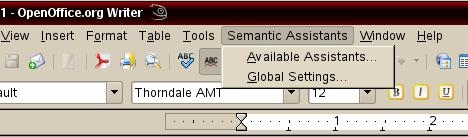
\includegraphics[width=0.7\textwidth]{pictures/oomenu.jpg}
\end{center}

In this menu, the user can inquire about available services, which are
selected based on the client (here \emph{Writer}) and the language
capabilities of the deployed NLP services (described in service
metadata, see Section~\ref{sec:owl}). The dynamically generated list
of available services is then presented to the user, together with a
brief description, in a separate window, as shown in
Figure~\ref{fig:oolist}. Note that the integration of a new service
does not require any changes on the client side---any new NLP service
created and deployed by a language engineer is dynamically discovered
through its OWL metadata maintained by the architecture and so becomes
immediately available to any connected client.
\begin{figure}[htb]
  \centering
  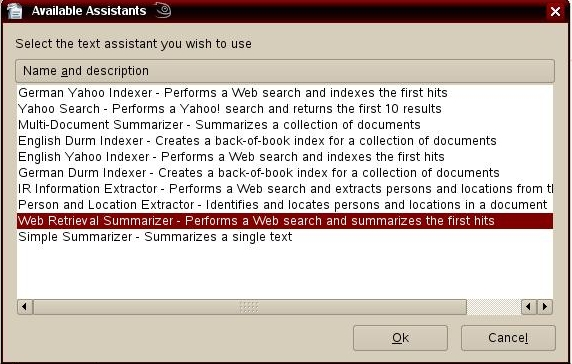
\includegraphics[width=0.5\textwidth]{pictures/oolist.jpg}
  \caption{List of available semantic assistants}
  \label{fig:oolist}
\end{figure}

The user can now select an assistant and execute it. In case the
service requires additional parameters, such as the length of a
summary to be generated, they are detected by our architecture through
the OWL-based service description and requested from the user through
an additional dialog window. An example, for the \emph{Web Retrieval
  Summarizer} assistant, is shown in Figure~\ref{fig:ooparams}.
\begin{figure}[htb]
  \centering
  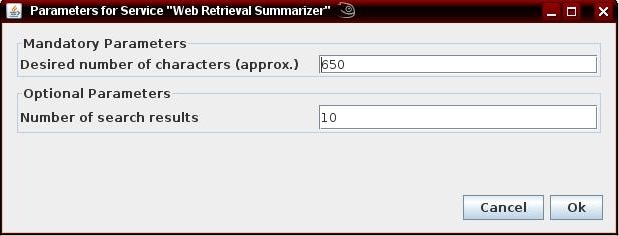
\includegraphics[width=0.5\textwidth]{pictures/ooparams.jpg}
  \caption{The parameters dialog, which appears when a Semantic
    Assistant requiring further input is invoked}
  \label{fig:ooparams}
\end{figure}
After the service is executed, the result is displayed in Writer depending on
the type of the server response: either as a new document, as annotations on
the existing document, or by opening an external viewer (e.g., a Web browser
for HTML documents).

\subsubsection{Side-Notes View}
The latest release of the OpenOffice.org Suite offer a new feature for text
annotation.  Depending on the annotation results received from GATE, the
Semantic Assistants Writer plug-in presents it in a sidenote manner (see
Figure~\ref{fig:sidenotes}).
\begin{figure}[htb]
  \centering
  %\vspace*{-9mm}
  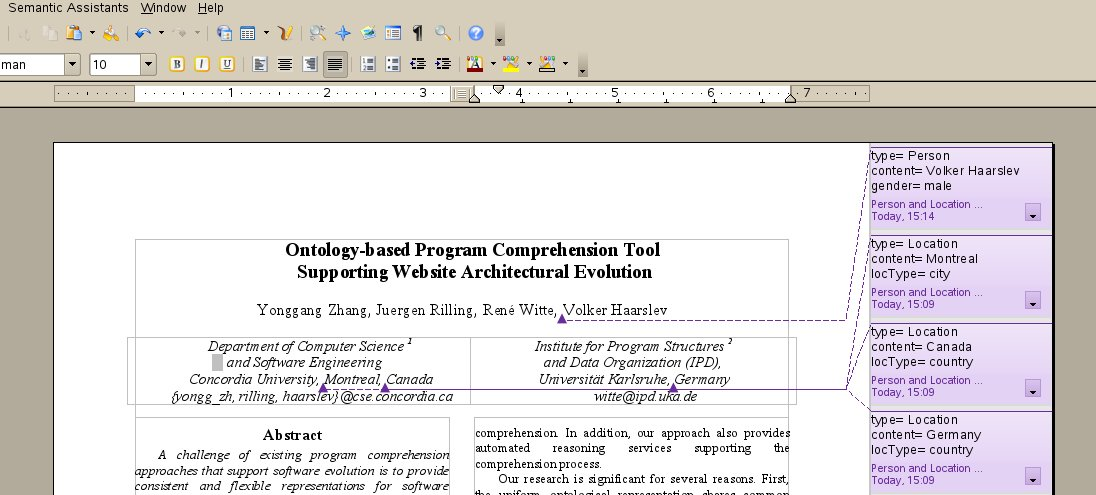
\includegraphics[width=0.8\textwidth]{pictures/sidenotes.jpg}
  \caption{Auto-Generated SideNotes Example}
  \label{fig:sidenotes}
  %\vspace*{-0.4cm}
\end{figure}

\subsubsection{New Document Creation}
\label{sec:doc-cre}
Creation of a new document comes handy when the output of an NLP service
corresponds to a complete document, or the result itself is indivisible. Some
examples are summarization or question-answering (see Figure~\ref{fig:oores}).

\begin{figure*}[htb]
  \centering
  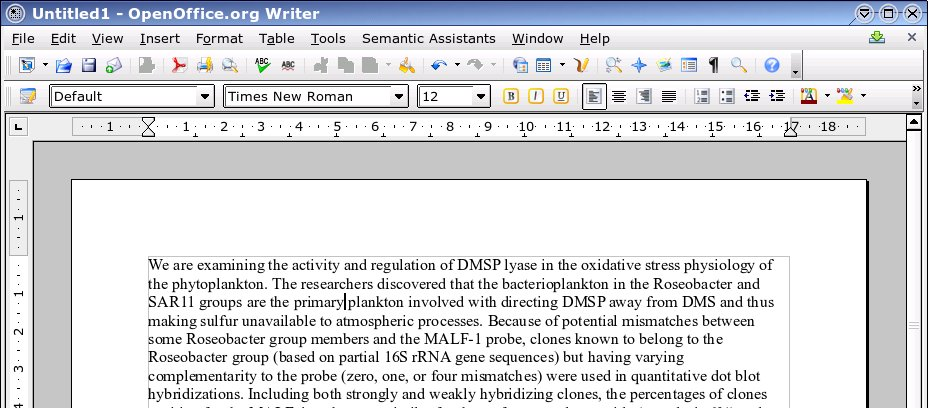
\includegraphics[width=0.8\textwidth]{pictures/ooresult_clip.jpg}
  \vspace*{-2mm}
  \caption{NLP services can also create a completely new document as a
  result (e.g., through summarization)}
  \label{fig:oores}
\end{figure*}

\subsubsection{Annotation Highlighting}
Besides text annotation, we offer the option for enabling/disabling annotation
highlighting for text that has been processed by GATE. This option can be
found under the Semantic Assistants menu in ``Global Settings.''  See
Figure~\ref{fig:highlight} for an example.

\subsubsection{Filter Empty Features}
This option found under the Semantic Assistants menu in ``Global Settings'' (shown
in Figure~\ref{fig:oosettings}) allows the ability to enable/disable filtering of
empty valued features in side-nodes. This can be useful to avoid cluttering or aid
debugging annotations respectively.

\subsubsection{Show Annotation Content}
This option in the ``Global Settings'' dialog can be used to include/exclude
the annotated content within the side-note. This can be used as an alternative
to annotation highlighting.

\begin{figure}
  \centering
  %\vspace*{-9mm}
  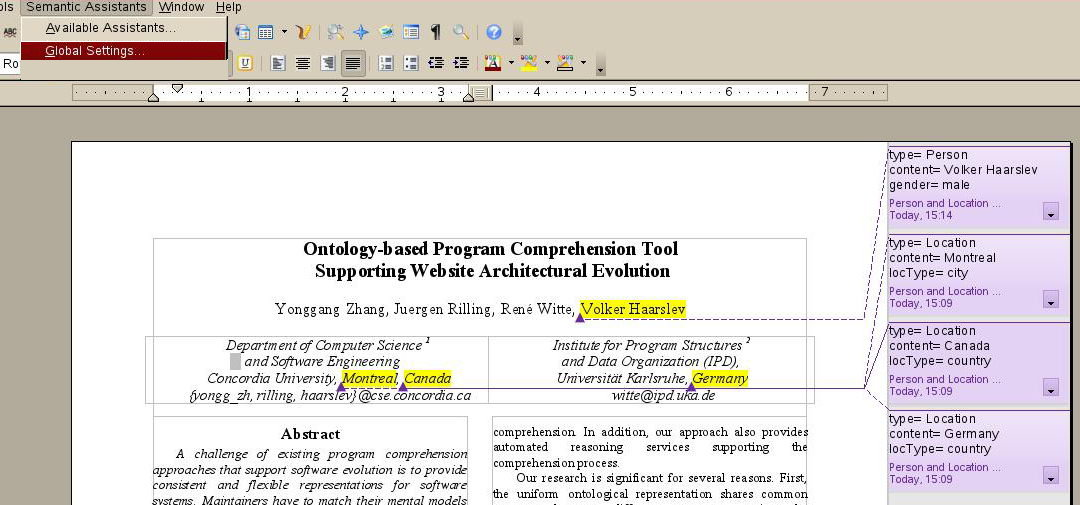
\includegraphics[width=0.8\textwidth]{pictures/highlighting.jpg}
  \caption{Highlighted Annotations Example}
  \label{fig:highlight}
  %\vspace*{0.5cm}
\end{figure}

\begin{figure}[htb]
\begin{center}
  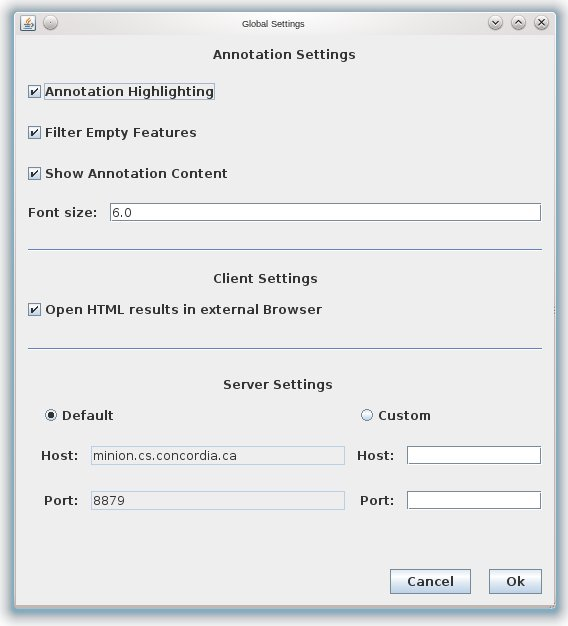
\includegraphics[width=0.5\textwidth]{pictures/oosettings.jpg}
  \caption{Configuration Dialog}
  \label{fig:oosettings}
\end{center}
\end{figure}

\subsubsection{Annotation Font Size}
As shown in Figure~\ref{fig:oosettings}, the font size of annotations can be changed
prior to invoking assistants. Due to the fixed width of side-notes, customizing the
size can ease readability of features.

\subsubsection{Browser Handling of HTML Results}
Instead of returning annotations, some pipelines produce HTML documents. The
``Open HTML results in external Browser'' option shown in Figure~\ref{fig:oosettings},
allows OpenOffice to invoke a local browser to display these results.

\subsubsection{Server Settings}
Another option found under the Semantic Assistants menu in ``Global
Settings.'' is \emph{Server Settings}.  There the user is able to specify the
Server information (Host and Port) of a local or distant server.

\subsection{Installation}
\label{subsec:oo-inst}
The OpenOffice.org plug-in can be found in
\url{SemanticAssistants/Clients/OpenOffice} and it is compatible with 
OpenOffice versions greater than 2.0.4. To use it, do the following:

\begin{enumerate}
  % TODO: what about the OO SDK installation? 
  % Is it needed for running the plug-in?

  \item Start OpenOffice.org Writer and ensure the right Java VM is
  used. Go to \emph{Tools $\rightarrow$ Options}. Under
  \emph{OpenOffice.org} you will find a \emph{Java} item. There, you
  can specify JREs. If it is not already there, add the currently used
  Java version.
  
  % should add screenshots for this
  \item Go to \emph{Tools $\rightarrow$ Extension Manager}. Click the
    \emph{Add$\ldots$} button on the bottom. Navigate to your local
    copy of the \sa\ architecture and then to
    \texttt{Clients/OpenOffice}. Select the file
    \texttt{SemassistOpenOfficePlugIn.oxt} and click \emph{Open}.

  \item Leave the dialog and open a new text document. You should have
    a new menu bar entry labeled \emph{Semantic Assistants}. Now you
    can run services on the current document (remember the server must
    be running to be able to query or execute language services).
\end{enumerate}


\subsection{Development Notes}
\label{sec:oo-spec}
In this section, we provide further technical details on our plug-in
for developers interesting in enhancing or modifying it.

\subsubsection{Compiling the Plug-in}
If you want to build the plugin yourself, follow these steps:
\begin{itemize}
  \item cd to the \url{Clients/OpenOffice} directory.

  \item Type \texttt{ant run}, or \texttt{ant run-gui}. Note that the
    client-side abstraction layer must have already been built and
    packaged. Both \texttt{ant run} and \texttt{ant run-gui} provide
    an UNO package named \url{SemassistOpenOfficePlugIn.oxt}. Both
    targets additionally copy it to \url{~/Documents/uno-components}.
    If \texttt{ant run-gui} is issued the OpenOffice.org
    \emph{Extension Manager} will pop up and prompt the user to
    install the extension.  If \texttt{ant run} is issued the above
    process is automated.  After the installation, OpenOffice Writer
    starts with the plug-in installed.

    \textbf{Note:} you can also manually add the plug-in from within
    OpenOffice (skip this step if you already used the \emph{run} or
    \emph{run-gui} target): Go to Tools, Extension Manager. Select
    \emph{My Extensions}, then click \emph{Add...} on the
    right. Choose the UNO package (available in
    \url{~/Documents/uno-components} if you used the \emph{deploy}
    target for ant).
\end{itemize}

\subsubsection{OpenOffice.org Plug-in Specifics}
Every plug-in has to include a \emph{description.xml} that describes the 
package's meta details like publisher, license, download url and version dependencies.
See \href{http://wiki.services.openoffice.org/wiki/Documentation/DevGuide/Extensions/Description_of_XML_Elements}{OpenOffice Developer's Guide}
for a list of available elements. The plug-in package also includes a
\emph{META-INF} directory, which contains a file called
\emph{manifest.xml}. This XML file lists the elements that come with
this plug-in;  The concrete manifest file for our plug-in is listed in
Figure~\ref{list:manifest}.  We can see that it defines three
\emph{file-entry} elements specifying the type and location of the
following files:
\begin{figure}[tb]
\centering
\begin{lstlisting}[language=XML,numbers=left,xleftmargin=8mm,columns=flexible]
<?xml version="1.0" encoding="UTF-8"?> 
<!DOCTYPE manifest:manifest PUBLIC 
"-//OpenOffice.org//DTD Manifest 1.0//EN" "Manifest.dtd"> 
<manifest:manifest 
 xmlns:manifest="http://openoffice.org/2001/manifest"> 
  <manifest:file-entry 
     manifest:media-type=
        "application/vnd.sun.star.configuration-data" 
     manifest:full-path="Addons.xcu"/> 
  <manifest:file-entry 
     manifest:media-type=
        "application/vnd.sun.star.configuration-data" 
     manifest:full-path="ProtocolHandler.xcu"/> 
  <manifest:file-entry 
     manifest:media-type=
        "application/vnd.sun.star.uno-component;type=Java" 
     manifest:full-path=
        "ProtocolHandlerAddon_java.uno.jar"/>
   <!-- Add any other plug-in required jar files here. -->
</manifest:manifest> 
\end{lstlisting}
\caption{The \emph{manifest.xml} file for our plug-in}
\label{list:manifest}
\end{figure}


\begin{description}
\item[\emph{Addons.xcu}.] This XML file defines how the plug-in should
  be integrated with OpenOffice.org. In our case, it contains a menu
  definition, specifying that the menu should only appear in the
  \emph{Writer} application. For each menu item, we specify which
  messages should be broadcast throughout the OpenOffice.org runtime
  system when the menu item is activated.
\item[\emph{ProtocolHandler.xcu}. ] This XML file specifies that the
  messages defined in \emph{Addons.xcu} should be handled by an object
  of a certain class. This class is provided in the Java archive and
  must adhere to a certain interface. 
\item[\emph{ProtocolHandlerAddon\_ java.uno.jar}.] This Java archive
  contains the actual functionality of the plug-in. It holds classes
  responsible for receiving the messages generated by the menu items,
  as well as classes responsible for the interaction with the
  client-side abstraction layer.
\end{description}


\subsubsection{Implementation Details}
A useful class called \url{UNOUtils} found in the \url{package
  info.semanticsoftware.semassist.client.openoffice.utils} contains most of
the OO-Writer feature implementations.  More specifically, the three methods in
Figure~\ref{list:ssb} implement a major part of the above described features
(Side-Notes, Highlighting and New Document Creation).

\begin{figure}
\centering
\begin{lstlisting}[language=Java,numbers=left,xleftmargin=8mm,columns=flexible]

private static XComponent CreateNewDocument( XDesktop xDesktop, 
					     String sDocumentType )
{
	...
}

private static void AnnotateField( Annotation annotation )
{
	...
	// Use the text document's factory to create an Annotation text field
	XTextField xAnnotation = (XTextField) UnoRuntime.queryInterface(
		XTextField.class, mxDocFactory.createInstance(
		"com.sun.star.text.TextField.Annotation" ) );
	
	// get the properties of the field
	XPropertySet xPropertySet = (XPropertySet) UnoRuntime.queryInterface( 
						XPropertySet.class, xAnnotation
);
	
	...
	
	// Highlight annotated field
        HighlightField();
}

private static void HighlightField()
{
....

}
\end{lstlisting}
\caption{Core methods implementing the OpenOffice Writer plug-in features are
  part of the \texttt{UNOUtils} class}
\label{list:ssb}
\end{figure}

%More details on how to compile and debug an OpenOffice plug-in can be found in Section~\ref{sec:debug}.
 
\subsubsection{Configure the OpenOffice Writer to Run in Debug Mode}
This Section describes how to configure the JAVA VM in OpenOffice Writer to accept incoming connection for a debugger.

\begin{enumerate}
  \item Open OpenOffice Writer
  \item Go to Tools, Options. Under \emph{OpenOffice.org}, there is a \emph{Java} item. Select it and then Click on the 
        \emph{Parameter} button. There the parameters when running the JAVA VM are set.
  \item To run in debug mode \emph{Assign} the following 2 parameters:
  \begin{itemize}
    \item \textbf{-X debug}
    \item \textbf{-Xrunjdwp:transport=dt\_socket,server=y,suspend=n,address=7081}
  \end{itemize}
  \item \textbf{Note: The} \emph{address=7081} \textbf{should be the consistent with the port set within the debugger}
  \item  Now OO Writer is ready to accept connections from the debugger
\end{enumerate} 


\section{Eclipse Plug-in}
Eclipse is not a single monolithic program, but rather a small kernel containing
a plug-in loader surrounded by hundreds of plug-ins. The behavior of each
plug-in in this architecture is stored in its code, and its dependencies and
services are declared in the plug-in's manifest file. On each Eclipse startup,
the plug-in loader scans all the available manifest files in the Eclipse
exclusive plug-in folder and then builds a structure containing this
information.

We used this characteristic of Eclipse architecture to integrate our Semantic
Assistants architecture into the Eclipse environment in form of a plug-in, in
order to offer various Natural Language Processing services. The Semantic
Assistants Eclipse plug-in is basically a Java archive (JAR) file that ships
with its own specific content and a description file to introduce itself to the
Eclipse plug-in loader. 

\subsection{Features}
Once the Semantic Assistants plug-in is installed, it creates a new menu entry
in the Eclipse menu toolbar. A user can inquire about the available services
from the ``Available Assistants'' item and modify the connection settings to the
Semantic Assistants server by selecting the second item.
\begin{figure}[htb]
\begin{center}
  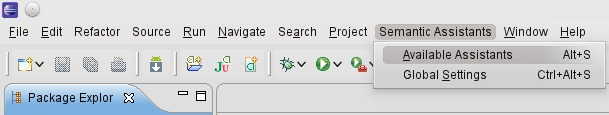
\includegraphics[width=1.0\textwidth]{pictures/eclipse_menu.jpg}
  \caption{Semantic Assistant Menu in Eclipse}
  \label{fig:eclipse_menu}
\end{center}
\end{figure}
\subsubsection{Available Assistants}
Selecting the ``Available Assistants'' item from Semantic Assistants menu will
open a file selection dialog. The file selection dialog allows the user to
select the desired files, folders and even complete projects to send to the
server as inputs to an NLP service. For more convenience, you can type an arbitrary extension like ``java'' or ``xml'', in the ``File Format'' field to filter to file tree view. 

\begin{figure}[htb]
\begin{center}
  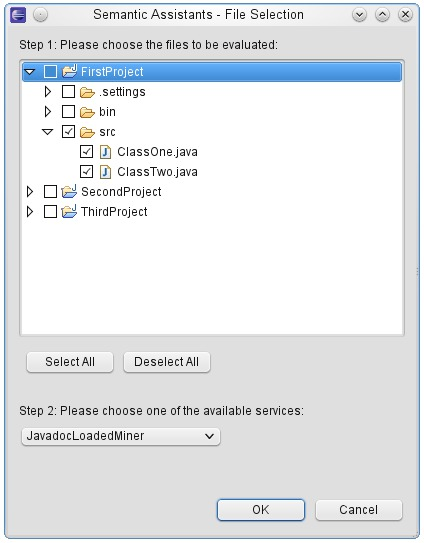
\includegraphics[width=0.5\textwidth]{pictures/eclipse_fileSelection.jpg}
  \caption{File Selection Dialog}
  \label{fig:eclipse_fileSelection}
\end{center}
\end{figure}

This dialog also lets the user to select an NLP service from a dynamically
generated list of services. This list is generated dynamically by selecting the
available services based on the client and the language capabilities of the
deployed NLP services. The server location where the service information are read from is presented just above the list as depicted in Fig \ref{fig:eclipse_services}. Note that the integration of a new service does not
require any changes on the client side - any new NLP service created and
deployed by a language engineer is dynamically discovered through its OWL
metadata maintained by the architecture and so becomes immediately available to
any connected client.

\begin{figure}[htb]
\begin{center}
  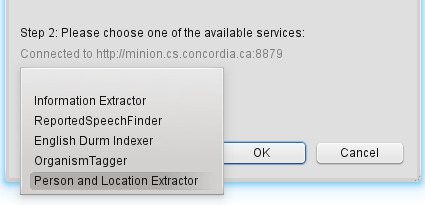
\includegraphics[width=0.5\textwidth]{pictures/eclipse_services.jpg}
  \caption{A List of Available NLP Services}
  \label{fig:eclipse_services}
\end{center}
\end{figure}

Upon selecting the resource files and the desired service, the user can execute
the selected service on the checked files in the tree. Consequently, the user will be informed about the status of the execution in the ``Semantic Assistant Status'' view. A successful execution of the selected NLP service, will let the user know on how to view the results. If the service execution fails, a description of the occurred error will be shown to the user and invocation will be aborted.

Now, let's look at how different types of outputs are handled in the plug-in:

\paragraph{Annotations.}
Annotations retrieved from a successful service invocation are being shown to the user in an
Eclipse view part called ``Semantic Assistants'' view. In the mentioned view, a
table will be dynamically generated that contains
all the parsed annotation instances. In Figure~\ref{fig:eclipse_saView} the
result of an execution of the ``Person and Location Extractor'' service on two
sample classes is shown.
\begin{figure}[htb]
\begin{center}
  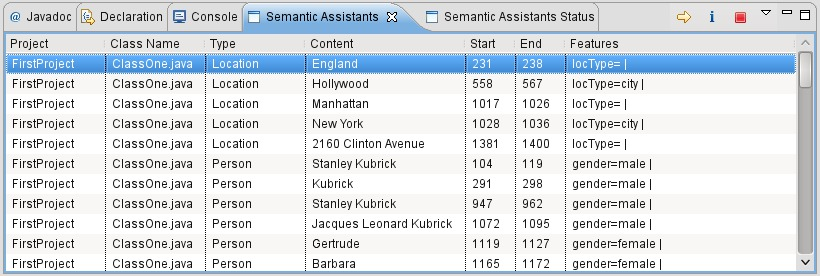
\includegraphics[width=1\textwidth]{pictures/eclipse_saView.jpg}
  \caption{Semantic Assistants View}
  \label{fig:eclipse_saView}
\end{center}
\end{figure}

This table can be sorted by different criteria through clicking on each column
title. Additionally, by double-clicking on each row in the table, the selected
annotation will appear with a graphical representation attached to the
corresponding resource. For instance, in Figure~\ref{fig:eclipse_annotation} the
JavadocMiner service has been invoked on a Java source code file. Some of the
annotations returned by the server bear a \emph{lineNumber} feature, which
attaches an annotation instance to a specific line in the java source file. Upon
double-clicking on the annotation instance in the Semantic Assistant view, the
corresponding resource - here, a .java file - will be opened in an editor and an
Eclipse warning marker will appear next to the line defined by the annotation
\emph{lineNumber} feature.

\begin{figure}[htb]
\begin{center}
  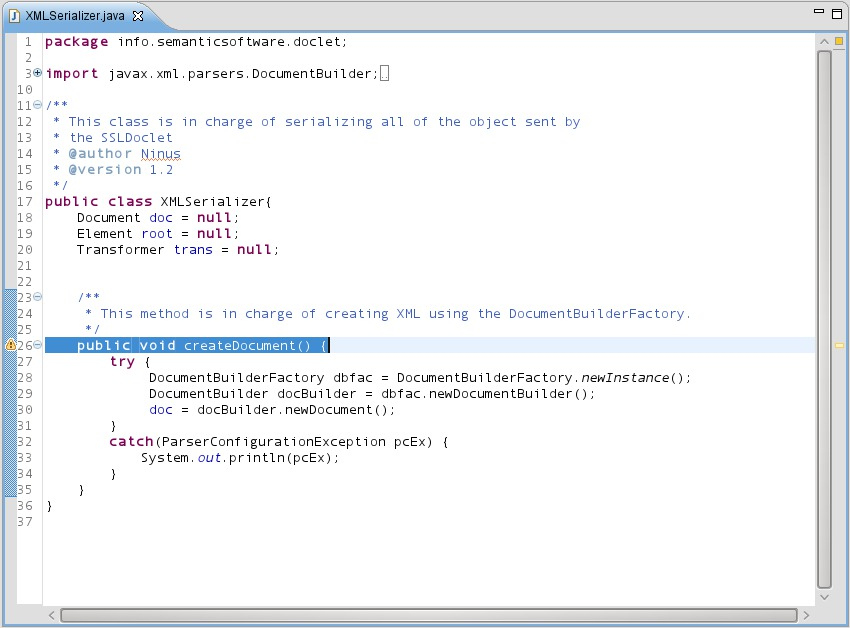
\includegraphics[width=1\textwidth]{pictures/eclipse_annotation.jpg}
  \caption{A Semantic Annotation}
  \label{fig:eclipse_annotation}
\end{center}
\end{figure}

\paragraph{Boundless Annotations.}
Boundless Annotations are a special kind of Annotations that adhere to a whole document and thus have no start and end offset. The plug-in parses the annotation results, and then inserts the content of the annotations in a new document and opens it in a new editor inside the Eclipse environment.

\paragraph{Documents.}
Documents received from the server response carry a URL property where defines where they are located. The plug-in retrieves the URLs and inserts them into a new document that opens up in a new editor inside the Eclipse environment.

\paragraph{Files.}
When a file output type is received by the plug-in, it will try to open it up in a web browser. In Eclipse, users can configure whether they want to open URLs in the Eclipse built-in web browser or any other ones in the file system. Whichever defined as the default behavior in Eclipse by the user, will be used by the plug-in to present the result file to the user. In this case, a log message will be shown to the user in the ``Semantic Assistants Status'' view to inform the user that the file is opened in his browser.

\subsubsection{Global Settings}
The second option found under the Semantic Assistants menu is the ``Global
Settings'' item. By clicking on this menu item, a dialog as depicted in Figure \ref{fig:eclipse_settings} is shown to the user that lets him choose a preferred server from a list of pre-defined values or add a custom server to the settings file. The values are provided in the Semantic Assistants global preference file described in \ref{sec:pref_management}. If the preference file gets accidentally deleted, a default preference file will be created by the plug-in but the eclipse-specific settings will be lost.
\begin{figure}[htb]
\begin{center}
  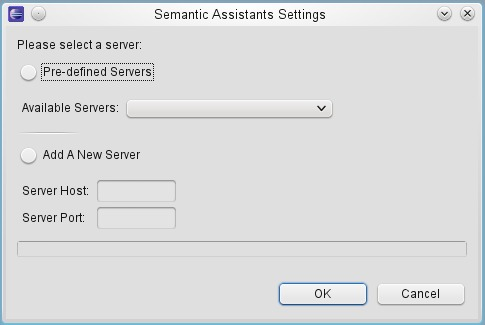
\includegraphics[width=0.6\textwidth]{pictures/eclipse_settings.jpg}
  \caption{Semantic Assistants Server Settings Dialog}
  \label{fig:eclipse_settings}
\end{center}
\end{figure}

\subsection{Installation}
\label{subsec:eclipse_install}
You can install the Semantic Assistants plug-in via the Eclipse software installer. To do so, first you have to add the Semantic Assistants software repository to your Eclipse list of software sites. In addition to installing the plug-in, adding the repository lets the Eclipse update manager to check for plug-in updates once available. Please carefully follow the steps listed below to install the Eclipse plug-in and refer to section \ref{trouble:eclipse_install} for installation troubleshooting.

\begin{enumerate}
  \item Select Help $\rightarrow$ Install New Software to open the Eclipse software installer.
  \item Press the ``Add'' button in the dialog, to add the Semantic Assistants repository.
  \item In the new dialog depicted in Fig \ref{fig:eclipse_install}, type ``\texttt{Semantic Assistants}'' and\\ ``\texttt{http://sa-eclipse.semanticsoftware.info}'' in ``Name'' and ``Location'' fields, respectively, and press ``OK''.
  \item The Semantic Assistants repository should now be added to your Eclipse list of software sites as seen in Fig \ref{fig:eclipse_install2}. From the loaded softwares, check the Eclipse plug-in and press ``Next''.
  \item Simply, follow the installation steps and let the installer restart the Eclipse application.
  \item The Eclipse plug-in loader will automatically load the plug-in for you. If the plug-in is installed
successfully, you should be able to see the Semantic Assistants menu added to
you toolbar.
\end{enumerate}

\begin{figure}[htb]
\begin{center}
  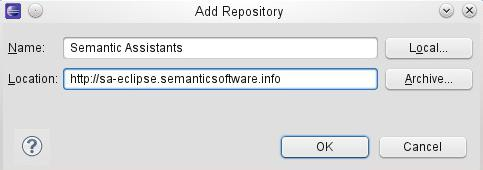
\includegraphics[width=0.6\textwidth]{pictures/eclipse_install.jpg}
  \caption{Adding Semantic Assistants Repository to Eclipse List of Software Sites}
  \label{fig:eclipse_install}
\end{center}
\end{figure}

\begin{figure}[htb]
\begin{center}
  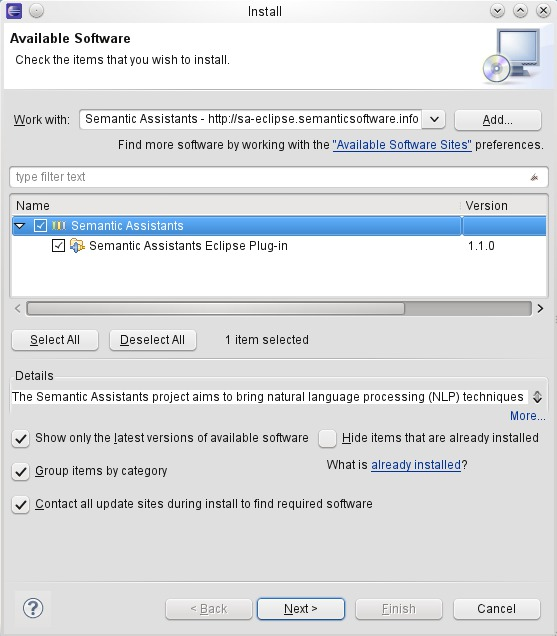
\includegraphics[width=0.6\textwidth]{pictures/eclipse_install2.jpg}
  \caption{Eclipse Software Installer Dialog}
  \label{fig:eclipse_install2}
\end{center}
\end{figure}

\subsection{Updating The Plug-in}
\begin{enumerate}
  \item Select Help $\rightarrow$ Check for Updates to open the Eclipse update manager.
  \item If there are any updates available for the Semantic Assistants plug-in, it will appear the in the update manager dialog as shown in Fig \ref{fig:eclipse_update}.
  \item Check the Semantic Assistants Eclipse plug-in from the list and press ``Next''.
  \item Follow the wizard steps and let the update manager restart your Eclipse for the updates to take place.
\end{enumerate}

\begin{figure}[htb]
\begin{center}
  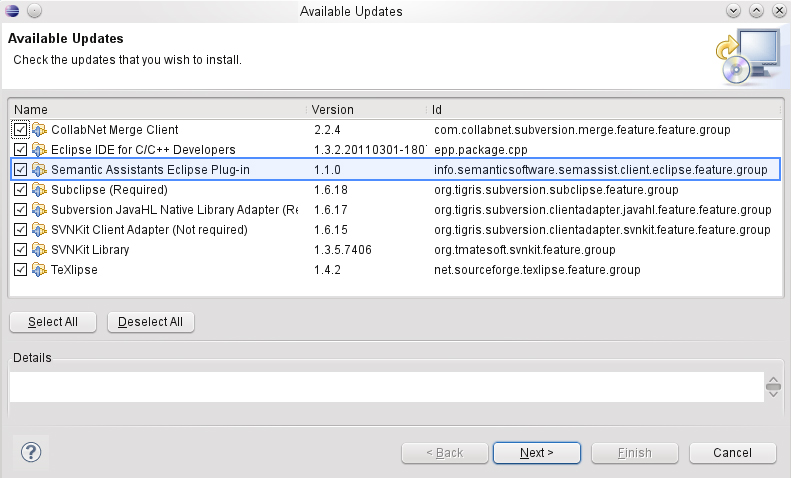
\includegraphics[width=1.0\textwidth]{pictures/eclipse_update.jpg}
  \caption{Updatin the Plug-in via Eclipse Update Manager}
  \label{fig:eclipse_update}
\end{center}
\end{figure}

\subsection{Development Notes}
\label{subsec:eclipse.development}
In this section, we provide further technical details on our plug-in for
developers interesting in enhancing or modifying it.

\subsubsection{Plug-in Source Directory Structure}
The Semantic Assistants plug-in uses Model-View-Controller pattern for its
implementation. Thus, most of the source code files are divided into different
packages related to their responsibilities. When you browse to
\url{src/info/semanticsoftware/semassist/client/eclipse/} folder, you see the
following structure:
\begin{enumerate}
\item\url{dialogs}: This folder contains the dialogs that are shown to the user
for interactions e.g. file selection. The classes inside this folder are the
codes for graphical user interfaces.
\item\url{handlers}: This folder contains the classes which play the controller
role in MVC pattern. Examples of these classes are dialog handlers and service
invocation jobs.
\item\url{model}: This folder contains the classes that provide data for
graphical user interfaces. These models are consumed by classes inside
\texttt{views} package.
\item\url{utils}: This folder contains utility classes e.g. logging feature.
\item\url{views}: This folder contains the source codes for Semantic Assistants
view parts. These are again graphical user interfaces but packaged differently
from dialogs.
\end{enumerate}

There is also another file called \url{Activator.java} in the source directory.
It is the main class of the plug-in that will be loaded initially and control
the plug-in's life cycle.

\subsubsection{Modifying the Plug-in}
If you want to modify the plug-in behavior or enhance it, follow these steps:
\begin{enumerate}
\item Open the Eclipse application.
\item Select File $\rightarrow$ New  $\rightarrow$ Project and under the
``Plug-in Development'' category select the ``Plug-in Project''.
\item A new plug-in project wizard will open up. Keep the EclipsePlugin name for
the project. Just below the project name there is a checkbox reading ``Use
Default Location''. Uncheck it and browse to the EclipsePlugin folder inside
where you've stored the Semantic Assistants folder.
\item Leave the other options untouched and press Finish.
\end{enumerate}

\begin{figure}[htb]
\begin{center}
  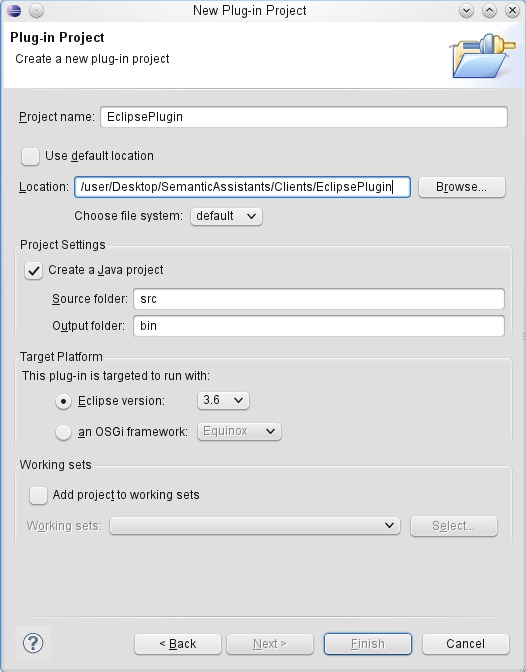
\includegraphics[width=0.5\textwidth]{pictures/eclipse_project_wizard.jpg}
  \caption{Eclipse New Plug-in Project Wizard}
  \label{fig:eclipse_project_wizard}
\end{center}
\end{figure}

\textbf{Note:} Remember you should manually copy the CSAL.jar file into you the
project's \texttt{lib} folder because it is a part of the project's dependency
and is defined in the classpath.

When the project is loaded in your workspace, feel free to play around. Browse
the source directory and add your development codes. To run your code, right
click on \texttt{plugin.xml} file and select Run As $\rightarrow$ Eclipse
Application.


\section{Extension for Mozilla Firefox and Mozilla Thunderbird} 

The Mozilla extension allows users to use Semantic Assistants in Mozilla Firefox and Mozilla Thunderbird and to leverage the \sa architecture within those applications. It is built on the extension platform that shared by Mozilla Firefox and Mozilla Thunderbird. Hence, it is a single extension that is compatible with both applications. The Mozilla extension aims to take the capabilities provided by Semantic Assistants and integrate them within the workflow of web browsing and of email reading and management. 

\subsection{Features}
\label{subsec:mozilla_features}

\subsubsection{User Interface Elements}
When the \sa Mozilla extension is installed, some new UI elements are added to the interface of the application. Firstly, a new ``Semantic Assistants" menu is added on the menu bar. Secondly, a new toolbar button is added to the primary toolbar of the application. (This toolbar button may be removed or relocated using Firefox/Thunderbird's built-in customization capabilities.) The toolbar button is actually a ``menu button," i.e., the left part is a button, and the right part opens a menu when clicked. Thirdly, a menu item is added to the contextual (right-click) menu of the principal content area of the application, that is, the browsing area in Firefox and the message body pane in Thunderbird. Lastly, a sidebar, which can be opened and closed, is added to the main window of the application. 

\paragraph{The ``Semantic Assistants" menu.} The ``Semantic Assistants" menu is 
located on the menu bar and opens a menu with the following three menu items: 
\begin{itemize} 
  \item Available Assistants... 
  \item Semantic Assistants Sidebar 
  \item Global Settings... 
\end{itemize} 

The ``Semantic Assistants" menu is shown in Figure~\ref{fig:mozilla_features_toolbar_menu_button}. 

\begin{figure}[htb]
  \centering
  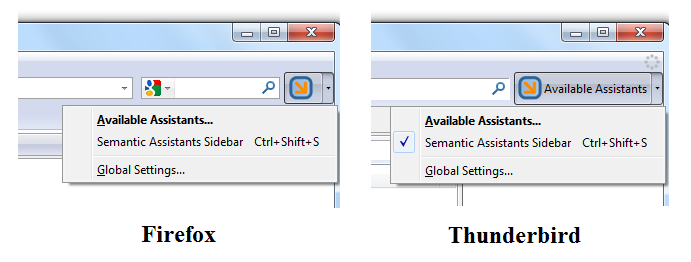
\includegraphics[width=0.8\textwidth]{pictures/mozilla_features_toolbar_menu_button.png}
  \caption{The toolbar menu button in Firefox and Thunderbird}
  \label{fig:mozilla_features_toolbar_menu_button}
\end{figure}

\paragraph{The ``Available Assistants" toolbar menu button.} The ``Available Assistants" menu button is located on the toolbar. The left side is a button and executes the ``Available Assistants" command (further elaborated later). Clicking the right side opens a menu that is identical to the ``Semantic Assistants" menu. 

\paragraph{The ``Available Assistants..." contextual menu item.} The ``Available Assistants" menu item appears on the contextual (right-click) menu of the main browsing area/page content area in Firefox and in the message body area in Thunderbird. Like the toolbar button, it also invokes the ``Available Assistants" command. 

\paragraph{The ``Semantic Assistants Sidebar".} The ``Semantic Assistants Sidebar" appears on the left side of the main window in Firefox and on the right side of the main window in Thunderbird. (The discrepancy is explained as follows. Firefox has built-in support for adding sidebars, and these appear on the left side of the main browsing window. Thunderbird, on the other hand, has no sidebars. Furthermore, the main inbox tab in Thunderbird already has a folder pane on the left side of the window. Hence, a custom sidebar was added, and it was placed on the right side of the main window.) 

The ``Semantic Assistants Sidebar" displays the results obtained from a service invocation to a Semantic Assistant. The following button in the Sidebar operate on the results: 
\begin{itemize} 
  \item \emph{Expand all}: Expands nodes of the results tree by one level.
  \item \emph{Collapse all}: Collapses all nodes of the results tree.
  \item \emph{Underline all}: Underlines all results in the tree in the page/message.
  \item \emph{Underline none}: Clears all the underlining in the page/message.
  \item \emph{Find previous underlined item}: Selects (highlights) the previous underlined text in the page/message.
  \item \emph{Find next underlined item}: Selects (highlights) the next underlined text in the page/message.
\end{itemize} 
The ``Semantic Assistants Sidebar" can be opened using the following ways: 
\begin{itemize} 
  \item \emph{Semantic Assistants} menu $\rightarrow$ \emph{Semantic Assistants Sidebar}
  \item \emph{Available Assistants} toolbar button menu $\rightarrow$ \emph{Semantic Assistants Sidebar}
  \item (in Firefox) \emph{View} menu $\rightarrow$ \emph{Sidebar} $\rightarrow$ \emph{Semantic Assistants Sidebar}
  \item (in Thunderbird) \emph{View} menu $\rightarrow$ \emph{Layout} $\rightarrow$ \emph{Semantic Assistants Sidebar}
  \item the keyboard shortcut \emph{Ctrl Shift S}
\end{itemize} 

The ``Semantic Assistants Sidebar" dialog is shown in Figure~\ref{fig:mozilla_features_sidebar}. 

\begin{figure}[htb]
  \centering
  % \includegraphics[width=0.8\textwidth]
  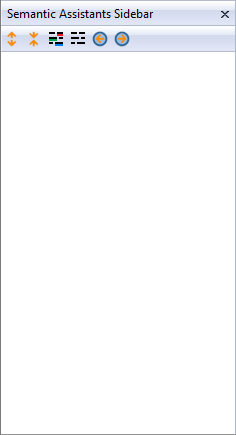
\includegraphics[totalheight=0.5\textheight]{pictures/mozilla_features_sidebar.png}
  \caption{The ``Semantic Assistants Sidebar" in Firefox and Thunderbird}
  \label{fig:mozilla_features_sidebar}
\end{figure}

\paragraph{The ``Global Settings" dialog.} The ``Global Settings" dialog allows the user to configure certain settings for the extension. These settings include:
\begin{itemize} 
  \item \emph{Server settings}: The user may choose to use the default defined server or to specify a custom server address. 
  \item \emph{Script settings}: The processing of the results is handled by a script run in Firefox/Thunderbird. If there are a lot of results or the page/message is long, the script may run for a long time. Firefox/Thunderbird has the built-in capability to prompt the user when a script has run for a given amount of time. By default, this amount of time is 20 seconds. The user may change this period if desired. Setting this setting to 0 signifies that the script will run forever. (Doing so, however, is not recommended, as the script may run for a very long time, and the only way to cancel would be to kill the whole application.)
\end{itemize} 
The ``Global Settings" dialog can be opened using the following ways: 
\begin{itemize} 
  \item \emph{Semantic Assistants} menu $\rightarrow$ \emph{Global Settings...}
  \item \emph{Available Assistants} toolbar button menu $\rightarrow$ \emph{Global Settings...}
\end{itemize} 

The ``Global Settings" dialog is shown in Figure~\ref{fig:mozilla_features_global_settings}. 

\begin{figure}[htb]
  \centering
  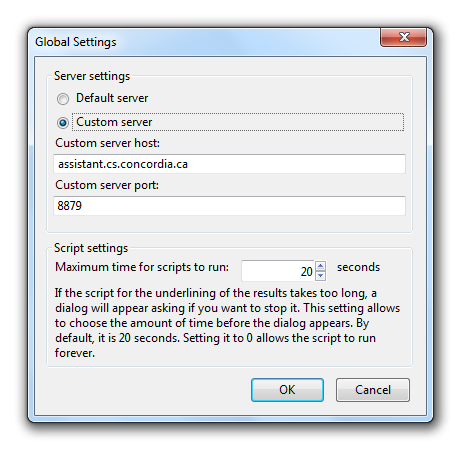
\includegraphics[width=0.8\textwidth]{pictures/mozilla_features_global_settings.png}
  \caption{The ``Global Settings" dialog in Firefox and Thunderbird}
  \label{fig:mozilla_features_global_settings}
\end{figure}

\subsubsection{Invoking a Semantic Assistant}
When the ``Available Assistants" command is invoked (either using the menu item in the ``Semantic Assistants" menu or in the menu of the toolbar button), a dialog entitled ``Available Semantic Assistants Services" appears (shown in Figure~\ref{fig:mozilla_features_available_assistants_dialog}), listing all available services from the server along with descriptions of each service. Upon the selection of a service, the extension sends the user-selected text in the page/message or, if text no selection was made, the whole text content of the page/message.

\begin{figure}[htb]
  \centering
  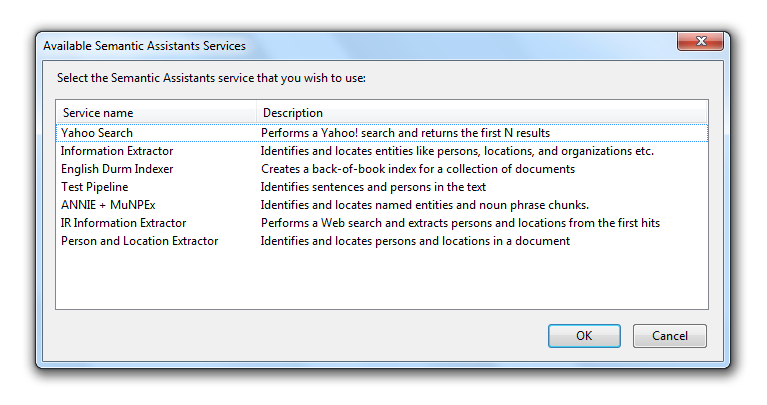
\includegraphics[width=1\textwidth]{pictures/mozilla_features_available_assistants_dialog.png}
  \caption{The ``Available Semantic Assistants Services" dialog in Firefox and Thunderbird}
  \label{fig:mozilla_features_available_assistants_dialog}
\end{figure}

When the results are returned by the server, two things happen. Firstly, the results are underlined in the page/message directly in the browsing area/message content area. Secondly, the ``Semantic Assistants Sidebar" is opened if it is not already so and displays the results. 

\subsubsection{Viewing the Results}
The results from the service invocation are underlined directly in the content of the page/message. The underlining is color-coded by annotation type to allow for better visual distinction. 

The results are also displayed in the ``Semantic Assistants Sidebar" in a tree format, grouped by annotation type, then by occurrences of a same word/phrase. 

The controls/buttons in the ``Semantic Assistants Sidebar" (mentioned previously in the ``User Interface Elements" section) can be used to manipulate the results tree, to underline all or no results and to go to the previous/next underlined result in the page/message.

Clicking on a node in the results tree will underline in the page/message the result or results represented by the node and all children of the node. For instance, if a leaf node of the tree is clicked in the Sidebar, the one result represented by that node is underlined. If an inner node of the tree is clicked in the Sidebar, then all the results represented by that node and all its child nodes are underlined. The ``Find previous underlined item" and ``Find next underlined item" buttons in the Sidebar will navigate only the currently underlined results. All put together, this allows to display precise subsets of the results, and to navigate through the occurrences of these results. 

The display of results within Firefox and Thunderbird is shown in Figure~\ref{fig:mozilla_features_firefox_window} and Figure~\ref{fig:mozilla_features_thunderbird_window_message_tab}.

\begin{figure}[htb]
  \centering
  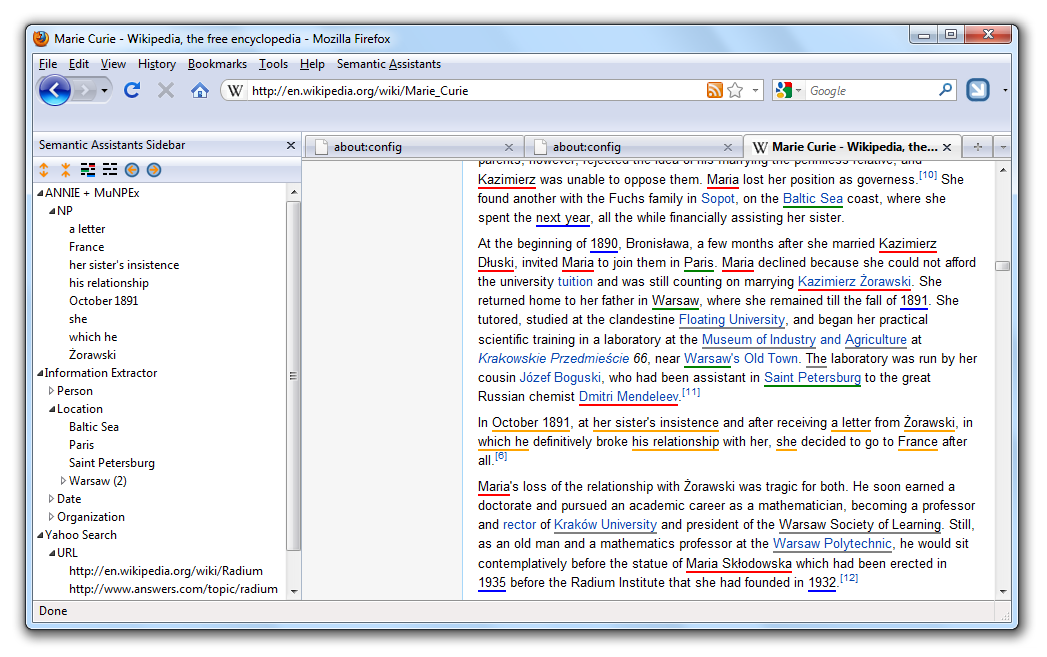
\includegraphics[width=0.95\textwidth]{pictures/mozilla_features_firefox_window.png}
  \caption{Results from a service invocation in Firefox}
  \label{fig:mozilla_features_firefox_window}
\end{figure}

\begin{figure}[htb]
  \centering
  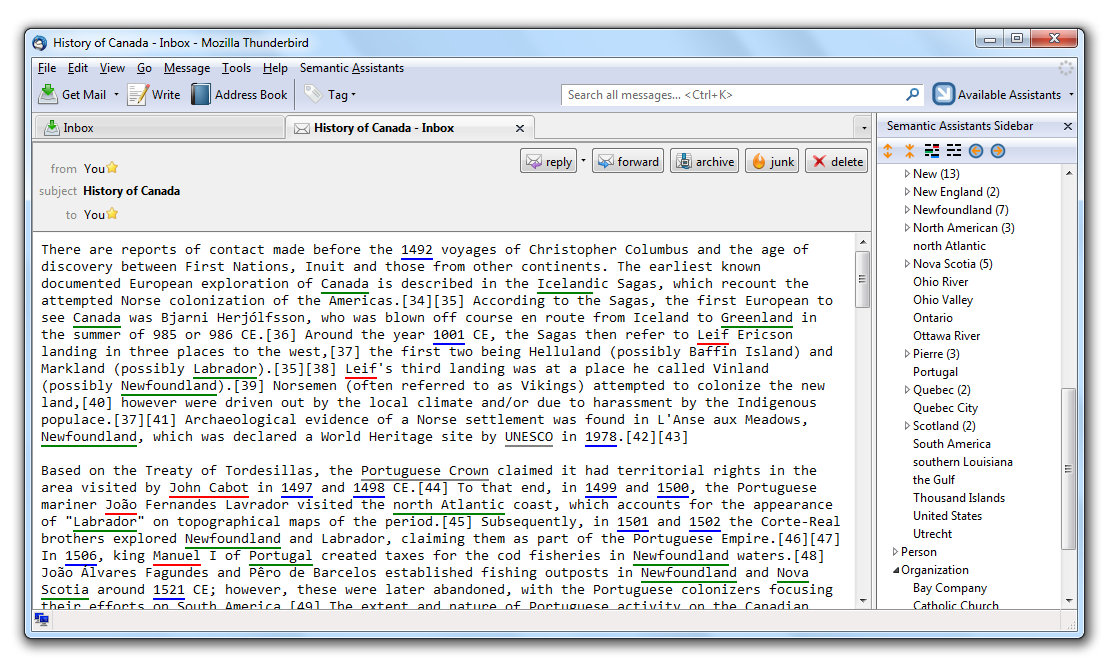
\includegraphics[width=0.95\textwidth]{pictures/mozilla_features_thunderbird_window_message_tab.png}
  \caption{Results from a service invocation in Thunderbird}
  \label{fig:mozilla_features_thunderbird_window_message_tab}
\end{figure}

\subsection{Installation}
\label{subsec:mozilla_installation}
The Mozilla extension comes in the form of a file with a .xpi extension. The .xpi file is installed in the standard manner in which extensions are installed in Mozilla Firefox and Mozilla Thunderbird. 

\subsubsection{Additional Notes about Prerequisites}
In addition to the basic prerequisites (refer to Chapter~\ref{chap:inst}), the following considerations should be noted: 
\begin{itemize}
  \item The Java runtime environment \emph{must} be the official Java Development Kit from Oracle (formerly from Sun). In certain Linux installations, OpenJDK is installed by default. This will not work for the Mozilla extension. (A ``java is not defined" error will occur.)
\end{itemize}

\subsubsection{Installation in Mozilla Firefox}
There are two methods to install the .xpi file in Firefox. The first method is to drag and drop the .xpi file into Firefox.
\begin{enumerate}
  \item Drag and drop the .xpi file into the main browsing area of the Firefox window.
  \item A dialog window entitled "Software Installation" appears. Click the ``Install Now'' button in the dialog.
  \item Restart Firefox.
\end{enumerate}
An alternate method is to use the file picker in Firefox.
\begin{enumerate}
  \item Select \emph{File $\rightarrow$ Open File...}.
  \item Navigate to the location of the .xpi file and choose it.
  \item A dialog window entitled "Software Installation" appears. Click the ``Install Now'' button in the dialog.
  \item Restart Firefox.
\end{enumerate}

\subsubsection{Installation in Mozilla Thunderbird 3.1.x and earlier}
Here is how to install the .xpi file in Thunderbird version 3.1.x and earlier. 
\begin{enumerate}
  \item Select \emph{Tools $\rightarrow$ Add-ons}.
  \item The Add-ons dialog opens. In the ``Extensions" section, at the bottom left, there is a button ``Install...". Click this button.
  \item Navigate to the location of the .xpi file and choose it.
  \item A dialog window entitled "Software Installation" appears. Click the ``Install Now'' button in the dialog.
  \item Restart Thunderbird.
\end{enumerate}

\subsubsection{Installation in Mozilla Thunderbird 5.0 and later}
Here is how to install the .xpi file in Thunderbird version 5.0 and later. 
\begin{enumerate}
  \item Select \emph{Tools $\rightarrow$ Add-ons}.
  \item The Add-on Manager opens. Near the top right, there is a button ``Tools for all add-ons" with a cog icon. Click this button.
  \item Click the ``Install Add-on from File" menu item.
  \item Navigate to the location of the .xpi file and choose it.
  \item A dialog window entitled "Software Installation" appears. Click the ``Install Now'' button in the dialog.
  \item Restart Thunderbird.
\end{enumerate}

If the installation succeeded, after the application restarts, the ``Semantic Assistants" menu in the menu bar should be visible, and the ``Available Assistants" toolbar button should be added to the toolbar. (For a full list of the UI elements of the extension, refer to section ~\ref{subsec:mozilla_features}.)

\subsection{Development Notes}
\label{subsec:mozilla_development}
This section details the layout of files in the extension, the overall architecture of the extension, and some specifics relating to Mozilla extension development. 

\subsubsection{A Brief Explanation of Mozilla Extensions}
An extension for the Mozilla platform is initially packaged in a .xpi file, which is simply a .zip file with the ``.xpi" file extension. Once the extension is ``installed" by the user, the contents of the .xpi file is extracted and placed in a newly created folder located in the ``extensions" folder within the Firefox/Thunderbird user profile folder. 

After the application restarts, the extension is loaded into memory, the installation of the extension to that specific user profile is complete.  

The Firefox/Thunderbird user profile folder is located at: 
\begin{itemize}
  \item Firefox \begin{itemize}
    \item On Windows XP: C:\textbackslash Documents and Settings\textbackslash WINDOWS\_ACCOUNT\_USER\_NAME \textbackslash Application Data\textbackslash Mozilla\textbackslash Firefox\textbackslash Profiles\textbackslash PROFILE\_FOLDER\_NAME
    \item On Windows Vista, 7: C:\textbackslash Users\textbackslash WINDOWS\_ACCOUNT\_USER\_NAME\textbackslash AppData\textbackslash Roaming \textbackslash Mozilla\textbackslash Firefox\textbackslash Profiles\textbackslash PROFILE\_FOLDER\_NAME
    \item On Linux: {\raise.17ex\hbox{$\scriptstyle\sim$}}/.mozilla/firefox/PROFILE\_FOLDER\_NAME
  \end{itemize}
  \item Thunderbird \begin{itemize}
    \item On Windows XP: C:\textbackslash Documents and Settings\textbackslash WINDOWS\_ACCOUNT\_USER\_NAME \textbackslash Application Data\textbackslash Thunderbird\textbackslash Profiles\textbackslash PROFILE\_FOLDER\_NAME
    \item On Windows Vista, 7: C:\textbackslash Users\textbackslash WINDOWS\_ACCOUNT\_USER\_NAME\textbackslash AppData\textbackslash Roaming \textbackslash Thunderbird\textbackslash Profiles\textbackslash PROFILE\_FOLDER\_NAME
    \item On Linux: {\raise.17ex\hbox{$\scriptstyle\sim$}}/.thunderbird/PROFILE\_FOLDER\_NAME or \char`\~/.mozilla-thunderbird/ PROFILE\_FOLDER\_NAME
  \end{itemize}
\end{itemize}
The profile's folder name (PROFILE\_FOLDER\_NAME) is by default a string of random characters followed by ``.default". If additional profiles are created, or if profiles are created manually, the name may be different. 

The user preferences of the extension are stored in a file called ``prefs.js" in the user profile folder. Conveniently, they can also be viewed and modified as follows. 
\begin{itemize}
  \item Firefox \begin{itemize}
    \item Type ``about:config" in the Location Bar and type Enter.
    \item If a warning message appears, click the button to continue.
  \end{itemize}
  \item Thunderbird \begin{itemize}
    \item Select \emph{Tools $\rightarrow$ Options...}.
    \item The Options dialog opens. In the ``Advanced" section, there is a button ``Config Editor...". Click this button.
    \item If a warning message appears, click the button to continue.
  \end{itemize}
\end{itemize}
A very long list of built-in Firefox/Thunderbird preferences and extension preferences is displayed. The preference in question can either be found manually, or the Filter at the top can be used to narrow down the list. Preferences can be modified by double-clicking on them. If it is a ``boolean" preference, its value is toggled. If it is a ``string" or ``integer" preference, a dialog box appears to allow the modification of the value. Changes are applied immediately. 

\subsubsection{File Layout}
The following covers the layout of the files of the extension. Inevitably, it will also include a brief overview of the general way a Mozilla extension works. The overall file layout can be seen in Figure~\ref{fig:mozilla_development_notes_file_layout}.

\begin{figure}[htb]
  \centering
  % \includegraphics[width=0.8\textwidth]
  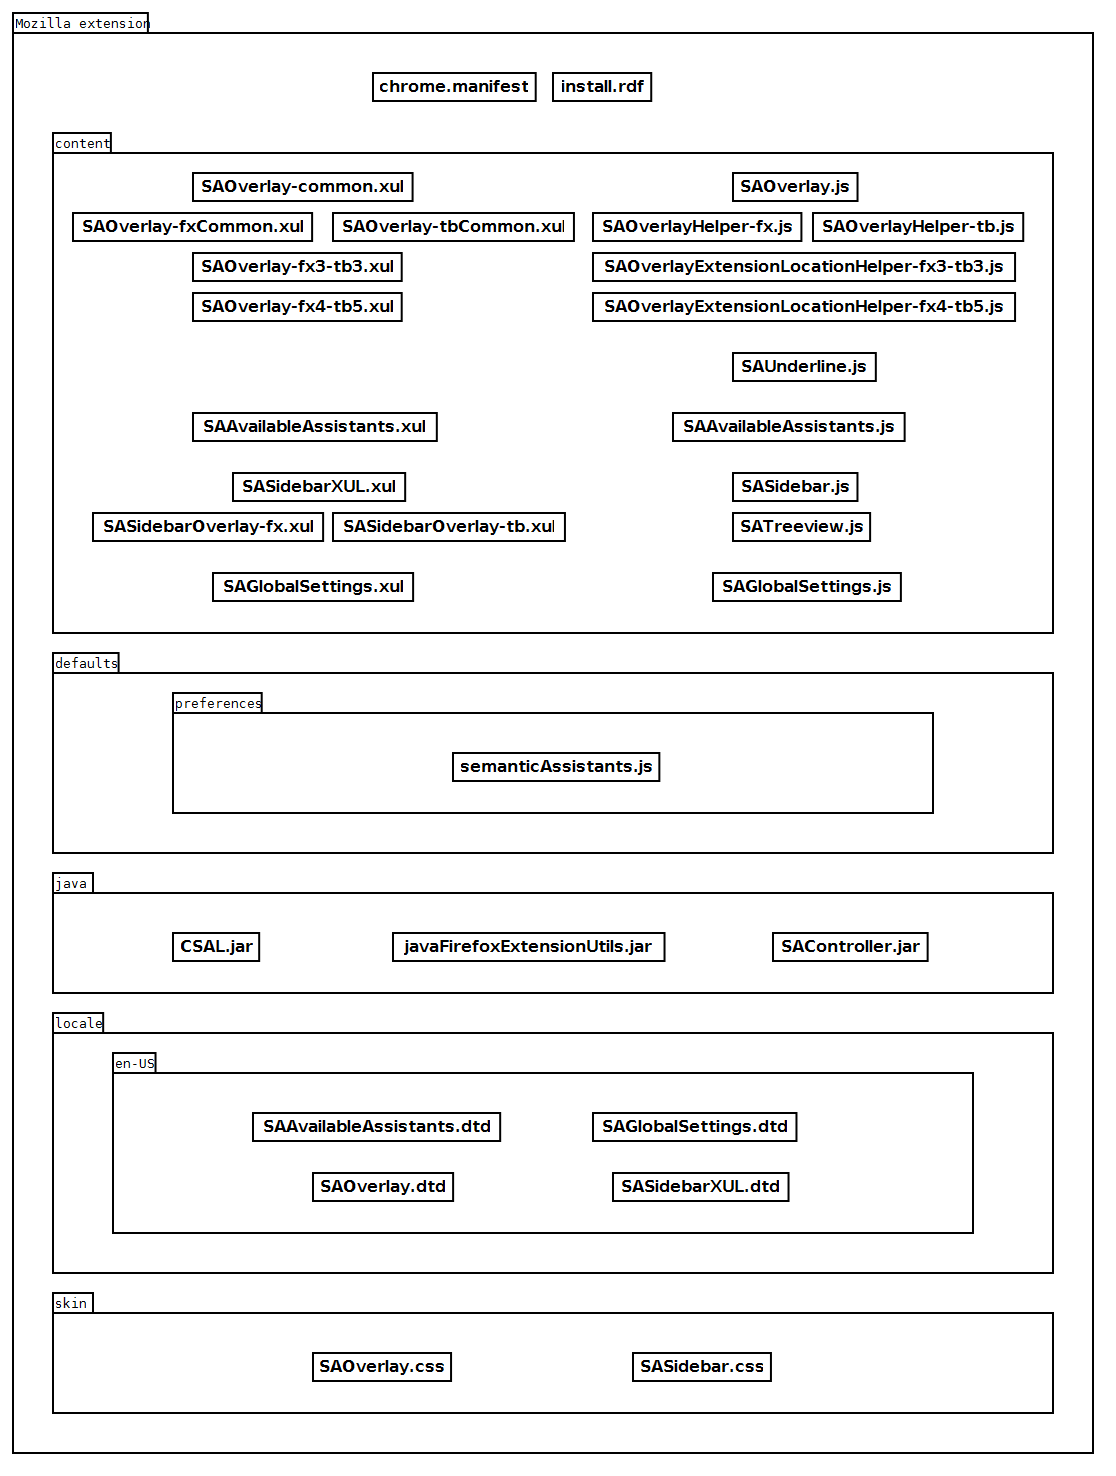
\includegraphics[totalheight=0.8\textheight]{pictures/mozilla_development_notes_file_layout.png}
  \caption{The file layout of the Mozilla extension}
  \label{fig:mozilla_development_notes_file_layout}
\end{figure}

\paragraph{Root folder} At the root of extension folder are two files called ``chrome.manifest" and ``install.rdf". The ``chrome.manifest" identifies the files contained within the extension and also allows to specify which files of the extension are to be loaded, depending on the application and the version of the application on which the extension is running (more on this later). The ``install.rdf" file defines various information about the extension, including the name of the extension (which becomes the name of the aforementioned extension folder), which applications and application versions that the extension is compatible with, and so on. 
\paragraph{The ``content" folder} This contains a series of XUL (.xul) files and JavaScript (.js) files. The XUL files define the user interface elements and behavior, such as windows, dialogs, menus, toolbar buttons. The JavaScript files contain the execution logic, and manipulation of user interface elements. 
\paragraph{The ``defaults" folder} Within the ``defaults" folder is the ``preferences" folder, which contains the default preferences for the extension. Upon installation of the extension, these defaults are set as the preferences in the Firefox/Thunderbird user profile (see above for specifics about preferences). 
\paragraph{The ``java" folder} The ``java" folder contains precompiled Java classes contained within .jar files. The ``CSAL.jar" is the same Client Side Abstraction Layer found in other clients. The ``javaFirefoxExtensionUtils.jar" file is a third-party utility which allows to grant full privileges to Java within a Mozilla extension. The ``SAController.jar" file is the Java component of the extension, which acts as a bridge between the JavaScript code and the CSAL and contains some additional execution logic. 
\paragraph{The ``locale" folder} The purpose of the ``locale" folder is to contain folders that contain files with localized strings used within the extension. These folders are named by specific languages' abbreviations (e.g., ``en-US"). 
\paragraph{The ``skin" folder} The ``skin" folder contains .css files that define layout and appearance properties image resource files for the icons and various UI elements within the extension.

\subsubsection{Compatibility Concerns}
There are differences in the extension between Firefox and Thunderbird. Furthermore, such differences also exist between Firefox 3.6.x and Firefox 4.0 as well as between Thunderbird 3.1.x and Thunderbird 5.0. (There was no Thunderbird 4.0.) This was because major changes were made to the Mozilla platform between those versions of the appliations. 

In order to enable the extension to be compatible with multiple version of Firefox as well as multiple versions of Thunderbird, certain measures were taken. 

Files of the extensions were split such that common code between applications/versions are kept within common files, while code that is different between applications/versions are separated into different versions of the files. The appropriate set of files is loaded for the right application and version. 

The aforementioned ``chrome.manifest" file, located at the root of the extension's folder structure, specifies the files to be loaded for the extension, depending on the application and application version on which the extension is running. Hence, for example, this allows for one file to be loaded for Firefox and another file to be loaded for Thunderbird. Another example would be for one file to be loaded for Firefox version 3.6 and earlier and another file to be loaded for Firefox version 4 and later. 

The files that need to have multiple versions are both the JavaScript files and the XUL files. The JavaScript code may differ between applications/versions due to differences in API. XUL files differ between applications (less for between versions of the same application) due to differences in the user interfaces (different elements, different naming, etc.).

Table~\ref{tab:mozilla_development_files_compatibility} shows which files are used depending on the application and the version of the application. 

\begin{table}[htb]
  \centering\small\sffamily
  \begin{tabular}{p{0.5\textwidth}@{\hspace*{4mm}}p{0.08\textwidth}@{\hspace*{4mm}}p{0.08\textwidth}@{\hspace*{4mm}}p{0.08\textwidth}@{\hspace*{4mm}}p{0.08\textwidth}}
    \toprule
    \textbf{} & \textbf{Fx 3.6.x} & \textbf{Fx 4.0+} & \textbf{Tb 3.1.x} & \textbf{Tb 5.0+} \\
    \midrule
    SAOverlay.js & x & x & x & x \\

    SAOverlayHelper-fx.js & x & x &  &  \\

    SAOverlayHelper-tb.js &  &  & x & x \\

    SAOverlayExtensionLocationHelper-fx3-tb3.js & x &  & x &  \\

    SAOverlayExtensionLocationHelper-fx4-tb5.js &  & x &  & x \\

    SAOverlay-common.xul & x & x & x & x \\

    SAOverlay-fxCommon.xul & x & x &  &  \\

    SAOverlay-tbCommon.xul &  &  & x & x \\

    SAOverlay-fx3-tb3.xul & x &  & x &  \\

    SAOverlay-fx4-tb5.xul &  & x &  & x \\

    SASidebarXUL.xul & x & x & x & x \\

    SASidebarOverlay-fx.xul & x & x &  &  \\

    SASidebarOverlay-tb.xul &  &  & x & x \\
    \bottomrule
  \end{tabular}
  \caption{Files loaded depending on application and version for compatibility}
  \label{tab:mozilla_development_files_compatibility}
\end{table}

\subsubsection{Extension Preferences}
The default preferences of the extension are defined in the folder ``defaults" in the ``preferences" subfolder in the file ``semanticAssistants.js". As previously mentioned, the current settings of those preferences are stored in a file called ``prefs.js" in the user profile folder. 

The preferences are: 

\begin{itemize}
  \item \emph{extensions.semanticAssistants.firstTimeRun} \begin{itemize}
    \item type: boolean
    \item default value: true
    \item This determines whether it is the first time that the extension is launched. If so, it adds the toolbar menu button to the application's main toolbar. 
  \end{itemize}
  \item \emph{extensions.semanticAssistants.installLocation} \begin{itemize}
    \item type: string
    \item default value: ""
    \item This stores the path of the extension. This is not a user preference; it is utilized internally when accessing the .jar files. It is set in the extension when the application's start up. 
  \end{itemize}
  \item \emph{extensions.semanticAssistants.serverCustomHost} \begin{itemize}
    \item type: string
    \item default value: ""
    \item This is a setting set by the user in the ``Global Settings" dialog. 
  \end{itemize}
  \item \emph{extensions.semanticAssistants.serverCustomPort} \begin{itemize}
    \item type: string
    \item default value: "8879"
    \item This is a setting set by the user in the ``Global Settings" dialog. 
  \end{itemize}
  \item \emph{extensions.semanticAssistants.serverDefaultOrCustom} \begin{itemize}
    \item type: integer
    \item default value: 0
    \item 0 for ``Default", 1 for ``Custom"
    \item This is a setting set by the user in the ``Global Settings" dialog. 
  \end{itemize}
\end{itemize}

\subsubsection{Overall Architecture}
The Mozilla extension is composed of three components: the principal component in JavaScript and XUL, the Java component of the extension (contained in the aforementioned ``SAController.jar" file), and the Client Side Abstraction Layer/CSAL (the ``CSAL.jar" file). A high-level representation of the overall architecture is shown in Figure~\ref{fig:mozilla_development_notes_overall_architecture_high_level}).
The main part of the extension is in JavaScript and XUL, as extensions for the Mozilla platform are written in JavaScript code, and the user interface is defined in XUL. A Java component exists in order for the JavaScript component to interoperate with the CSAL; it also adds additional execution logic, such as processing the results from the CSAL. Leveraging a feature in Firefox/Thunderbird called LiveConnect in addition to a third-party package to grant full privileges to Java within a Mozilla extension, the JavaScript code of the extension utilizes and calls the compiled Java code, which in turn utilizes and calls the CSAL. 

\begin{figure}[htb]
  \centering
  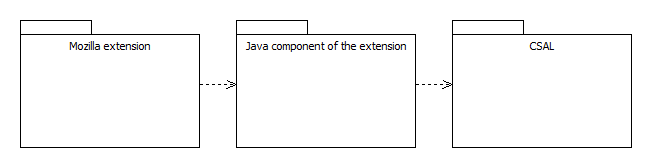
\includegraphics[width=0.8\textwidth]{pictures/mozilla_development_notes_overall_architecture_high_level.png}
  \caption{The overall architecture of the Mozilla extension at a high level}
  \label{fig:mozilla_development_notes_overall_architecture_high_level}
\end{figure}

The main class in the Mozilla extension component is ``SAOverlay" (defined in ``SAOverlay.js" under the ``contents" folder). This class communicates with the other classes in the component. Additionally, it is this class that calls the Java component. The facade for the Java component is the ``SemanticAssistantsController" class. Similarly, the ``SemanticAssistantsController" class is a controller, which coordinates the other classes in the Java component. The various classes of the Java component utilize classes contained within the CSAL. These dependencies are shown in Figure~\ref{fig:mozilla_development_notes_overall_architecture_more_detailed}.

\begin{figure}[htb]
  \centering
  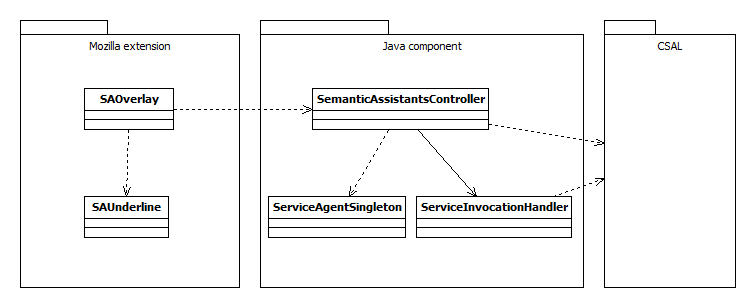
\includegraphics[width=0.8\textwidth]{pictures/mozilla_development_notes_overall_architecture_more_detailed.png}
  \caption{The overall architecture of the Mozilla extension showing some more details in terms of dependencies and showing some of the main modules}
  \label{fig:mozilla_development_notes_overall_architecture_more_detailed}
\end{figure}

\subsubsection{Main Mozilla Extension Component}
The main component of the Mozilla extension consists of a series of JavaScript classes and XUL files. The class diagram in Figure~\ref{fig:mozilla_development_notes_mozilla_extension_class_diagram} shows the main classes and their associations in the main Mozilla extension component as well as the classes called within the Java component. 

\begin{figure}[htb]
  \centering
  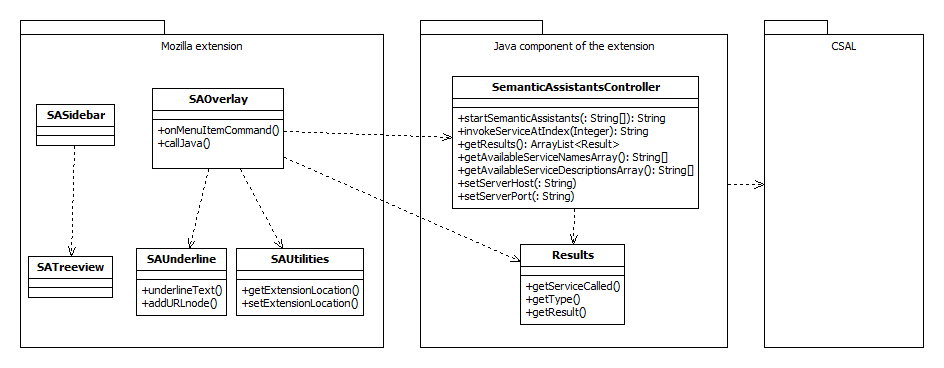
\includegraphics[width=0.95\textwidth]{pictures/mozilla_development_notes_mozilla_extension_class_diagram.png}
  \caption{Class diagram of the main Mozilla extension component}
  \label{fig:mozilla_development_notes_mozilla_extension_class_diagram}
\end{figure}

The main class is ``SAOverlay". When the user invokes the ``Available Assistants" command, it invokes the ``onMenuItemCommand" function in ``SAOverlay". This function obtains the user selection on the page/message, or the whole content of the page/message if no selection was made, and calls the function ``callJava" and passes the user selection. The ``callJava" function then obtains references to the Java classes in the Java component (``SAController.jar"). This is done using the feature called LiveConnect built into Firefox and Thunderbird. Additionally, the aforementioned third-party component ``javaFirefoxExtensionUtils.jar" is required to grant full privileges to the .jar files, as shown in Figure~\ref{list:mozilla_development_notes_main_mozilla_extension_component_jar_permissions}. The method ``startSemanticAssistants" of the ``SemanticAssistantsController" Java class is invoked, and the result returned is a list of available \sa NLP services (``Assistants"). Then, an XUL dialog ``SAAvailableAssistants.xul" is opened, prompting the user to choose an Assistant from the list. 

\begin{figure}
\centering
\begin{lstlisting}[language=Java,numbers=left,xleftmargin=4mm,columns=flexible]
callJava: function(userSelection, allText) {
    var extensionPath = SAOverlay.getExtensionLocation();
    
    var SAControllerJarPath = "file:///" + extensionPath + "/java/SAController.jar"; 
    var classLoaderJarPath = "file:///" + extensionPath + "/java/javaFirefoxExtensionUtils.jar";
    var CSALJarPath = "file:///" + extensionPath + "/java/CSAL.jar";
    
    urlArray = []; 
    urlArray[0] = new java.net.URL(SAControllerJarPath); 
    urlArray[1] = new java.net.URL(classLoaderJarPath);  
    urlArray[2] = new java.net.URL(CSALJarPath);  

    var cl = java.net.URLClassLoader.newInstance(urlArray);

    //set security policies with the policyAdd function defined below
    this.policyAdd(cl, urlArray);
    
    (...)
}, 

(...)

policyAdd: function(loader, urls) {
    try {
        var str = 'edu.mit.simile.javaFirefoxExtensionUtils.URLSetPolicy';
        var policyClass = java.lang.Class.forName(
            str,
            true,
            loader
            );
        var policy = policyClass.newInstance();
        policy.setOuterPolicy(java.security.Policy.getPolicy());
        java.security.Policy.setPolicy(policy);
        policy.addPermission(new java.security.AllPermission());
        for (var j = 0; j < urls.length; j++) {
            policy.addURL(urls[j]);
        }
    }
    catch(e) {
        alert(e+'::'+e.lineNumber);
    }
}
\end{lstlisting}
\caption{Granting full permissions to .jar files inside the extension in the \texttt{callJava} function in the \texttt{SAOverlay} class}
\label{list:mozilla_development_notes_main_mozilla_extension_component_jar_permissions}
\end{figure}

When the selection is made, another method ``invokeServiceAtIndex" of the ``SemanticAssistantsController" Java class is invoked, and upon successful return of the results, the ``getResults" method of the Java class is called to retrieve the results from the service invocation. Then, for each result within the results, an appropriate action is taken. For an ``annotation"-type result, the function ``underlineText" of the ``SAUnderline" JavaScript class is called; for a ``document"-type result, the function ``addURLnode" of ``SAUnderline" is called; for a ``file"-type result, no action is taken, as the Java code executes the opening the file. Save for a ``file"-type result, the ``Semantic Assistants" sidebar, which is the XUL file ``SASidebarXUL.xul", is opened to display the results. 

The sequence diagram in Figure~\ref{fig:mozilla_development_notes_mozilla_extension_sequence_diagram_main_scenario} shows the call sequence involved in the above main scenario of listing the available services and then of invoking a service. 
\begin{figure}[htb]
  \centering
  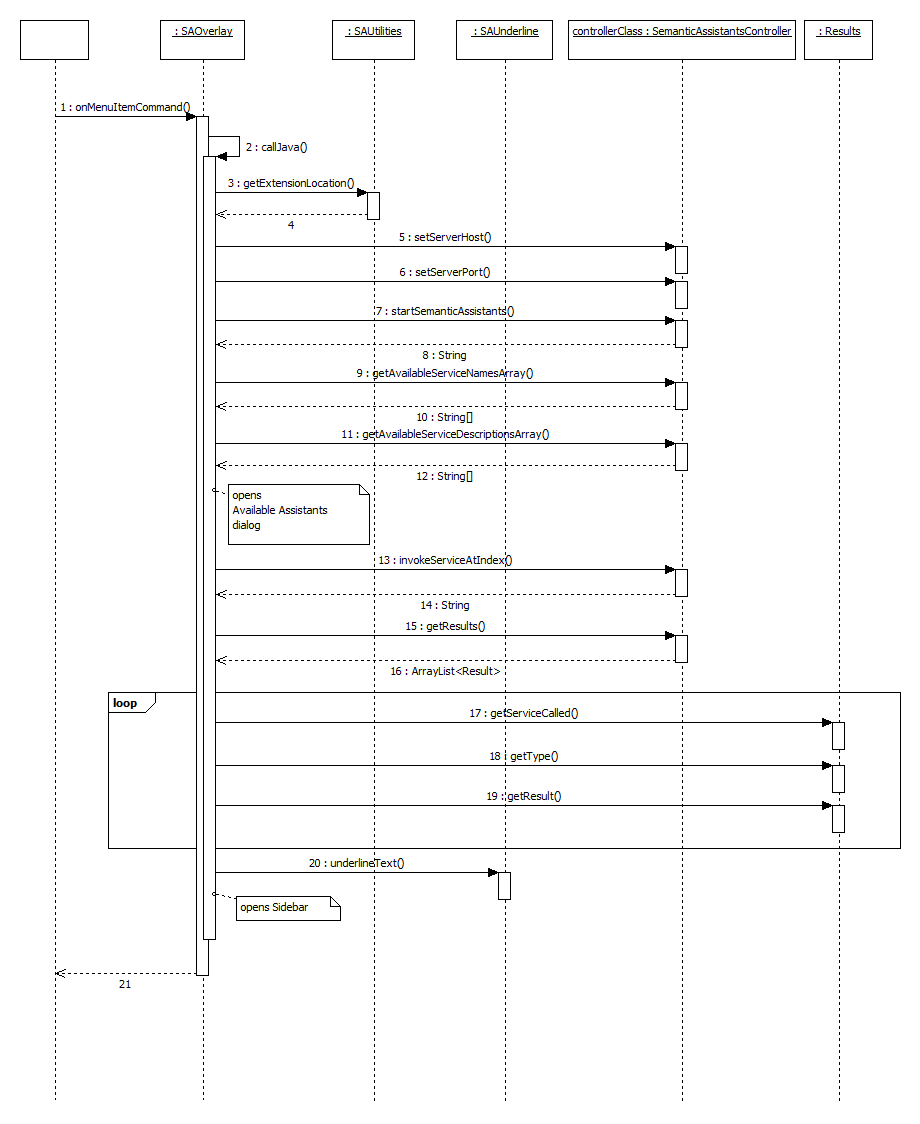
\includegraphics[totalheight=0.8\textheight]{pictures/mozilla_development_notes_mozilla_extension_sequence_diagram_main_scenario.png}
  \caption{Sequence diagram of the main Mozilla extension component for the main scenario}
  \label{fig:mozilla_development_notes_mozilla_extension_sequence_diagram_main_scenario}
\end{figure}

\subsubsection{Java Component}
The Java component consists of a series of Java classes packaged within a .jar file. The class diagram in Figure~\ref{fig:mozilla_development_notes_java_component_class_diagram} shows the principal classes and their associations in the Java component as well as some of the classes in the CSAL called from the Java component. 

\begin{figure}[htb]
  \centering
  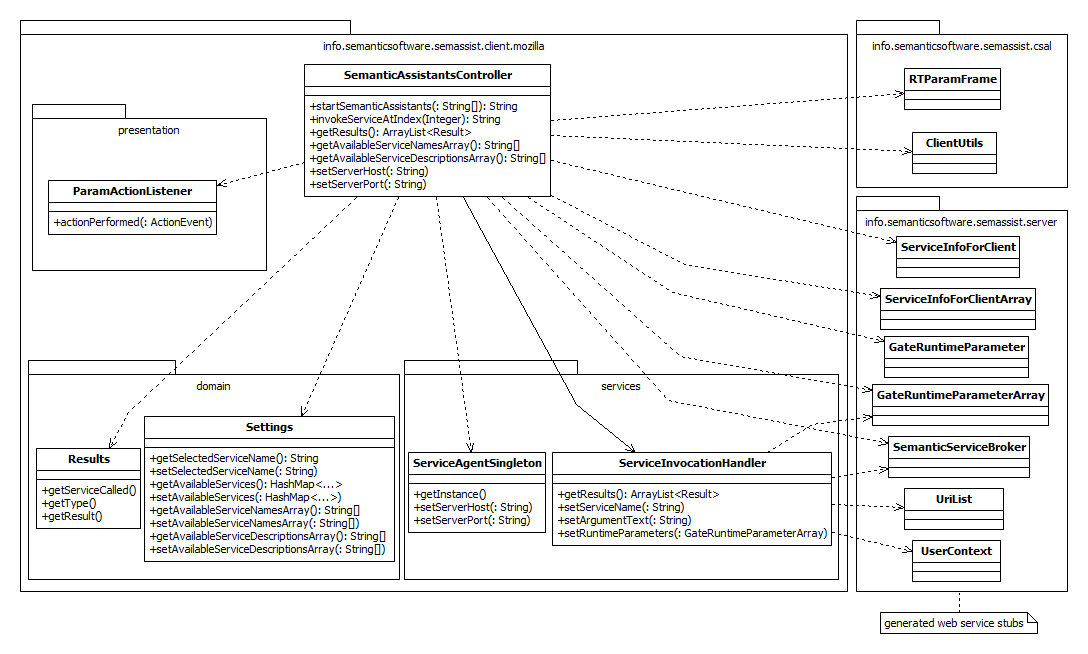
\includegraphics[width=0.95\textwidth]{pictures/mozilla_development_notes_java_component_class_diagram.png}
  \caption{Class diagram of the Java component}
  \label{fig:mozilla_development_notes_java_component_class_diagram}
\end{figure}

The main class is ``SemanticAssistantsController"; it is the facade class of the Java component packaged within ``SAController.jar" file and acts as a controller that calls and coordinates all other classes. 

\paragraph{The scenario of getting available services} The method ``startSemanticAssistants" of the ``SemanticAssistantsController" class is called. By calling ``getInstance" of ``ServiceAgentSingleton", a ``SemanticServiceBroker" instance is obtained. Calling ``getAvailableServices" of the latter returns a ``ServiceInfoForClientArray", which is a collection of the available services from the server. Then, these available services are stored in the ``Settings" class, as well as service names and service descriptions to be utilized by the main JavaScript component to display to the user. (A code snippet of this can be seen in Figure~\ref{list:mozilla_development_notes_java_component_get_available_services}.)

The sequence diagram in Figure~\ref{fig:mozilla_development_notes_java_component_sequence_diagram_get_available_services} shows the call sequence in the above scenario of obtaining the list of available services from the server. 

\begin{figure}
\centering
\begin{lstlisting}[language=Java,numbers=left,xleftmargin=4mm,columns=flexible]
SemanticServiceBroker agent = ServiceAgentSingleton.getInstance();
ServiceInfoForClientArray sia = agent.getAvailableServices();

List<ServiceInfoForClient> results = sia.getItem();
Iterator<ServiceInfoForClient> it = results.iterator();

(...)

while( it.hasNext() ) {
    ServiceInfoForClient info = it.next();
    availableServices.put( info.getServiceName(), info );
    (...)
}

(...)

Settings.setAvailableServices( availableServices );
\end{lstlisting}
\caption{Getting the available services in the the \texttt{startSemanticAssistants} method in the \texttt{SemanticAssistantsController} class}
\label{list:mozilla_development_notes_java_component_get_available_services}
\end{figure}

\begin{figure}[htb]
  \centering
  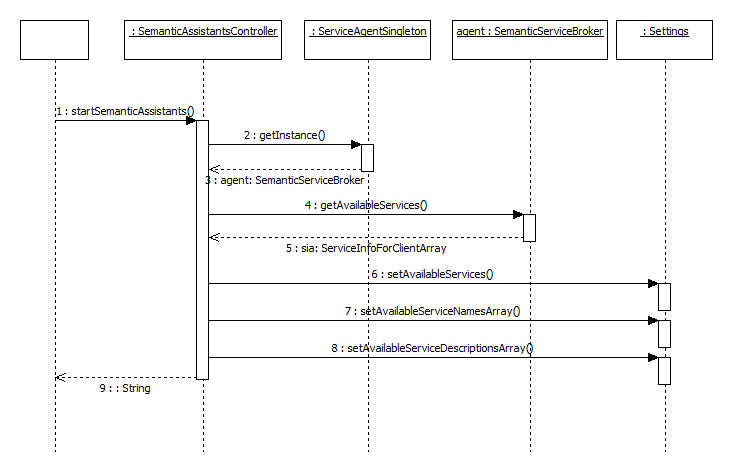
\includegraphics[width=0.95\textwidth]{pictures/mozilla_development_notes_java_component_sequence_diagram_get_available_services.png}
  \caption{Sequence diagram of the Java component for the scenario of getting available services}
  \label{fig:mozilla_development_notes_java_component_sequence_diagram_get_available_services}
\end{figure}

\paragraph{The scenario of invoking an available service} The method ``invokeServiceAtIndex" of the ``SemanticAssistantsController" class is called with the argument passed from the JavaScript code specifying which service was specified by the user. The name of the service, which is what is used to identify services, is determined. The method ``runSelectedService" is called, where the ``ServiceInfoForClient" corresponding to the service is retrieved from the list saving during the ``startSemanticAssistants" method call. 

If this service has parameters to be entered by the user, these parameters are retrieved based on the service and displayed in a ``JFrame" for the user to enter the required and optional parameters. 

A new ``GateRuntimeParameterArray" instance, containing the user input for the parameters if there were any, is passed to ``doRunSelectedService" method. In this method, the service name and text to be analyzed are set in a newly instantiated ``ServiceInvocationHandler" is instantiated, then ``getResults" is called. In this method, from ``ServiceAgentSingleton", ``SemanticServiceBroker" instance is obtained; ``invokeService" of this instance is called upon while passing the service name, the text to be analyzed, the parameters (if any), as well as other arguments. The result returned is a string which when processed by the ``getServiceResults" method of ``ClientUtils" yields a list of ``SemanticServiceResult" results. Then, each result is processed according to its result type. For example, for a "file"-type result, code is run to open the file in the Web browser; for a "annotation"- or "document"-type result, the result is set appropriately in the list of results returned to the JavaScript code, to be then processed by the main extension component. 

The sequence diagram in Figure~\ref{fig:mozilla_development_notes_java_component_sequence_diagram_invoke_service} shows the call sequence in the above scenario of invoking an available service from the server and obtaining the results. 

\begin{figure}[htb]
  \centering
  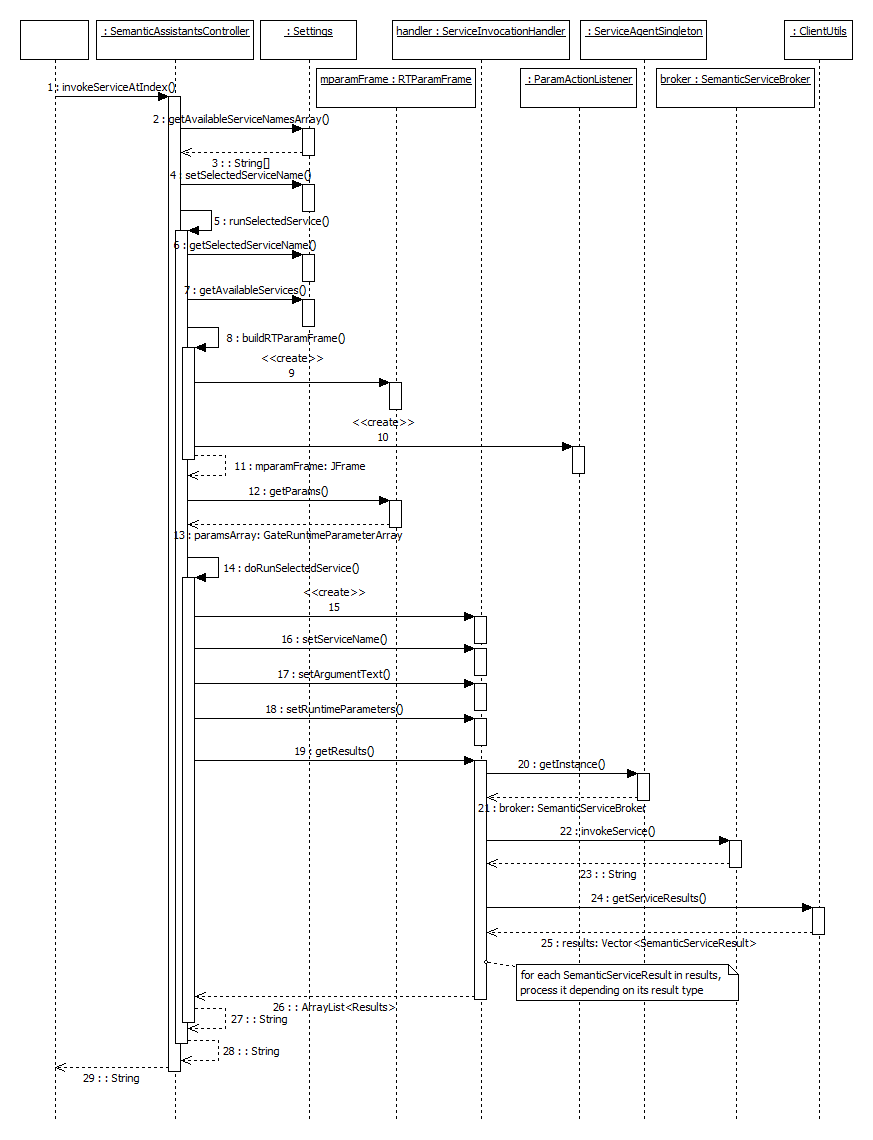
\includegraphics[totalheight=0.8\textheight]{pictures/mozilla_development_notes_java_component_sequence_diagram_invoke_service.png}
  \caption{Sequence diagram of the Java component for the scenario of invoking a service}
  \label{fig:mozilla_development_notes_java_component_sequence_diagram_invoke_service}
\end{figure}

\section{Wiki Integration}
Wikis are web-based software applications that allow users to collaboratively create and edit web page content, through a Web browser using a simplified syntax. The ease-of-use and ``open'' philosophy of wikis have brought them to the attention of organizations and online communities, leading to a wide-spread adoption as a simple and ``quick'' way of collaborative knowledge management. \sa architecture provides an extensible wiki connector component that allows a multitude of wiki engines to connect to a \sa server and employ various NLP services on their content.

The wiki connector component is designed regardless of what underlying wiki engine intends to use the NLP services within its environment. This means that the wiki component does not have any concrete wiki engine specifications hard coded in its implementation. Rather, it provides an extensible interface so that various wiki engines can be added to its architecture with little effort.

As a concrete application, we have developed the integration of \sa with the MediaWiki\footnote{MediaWiki, \url{http://www.mediawiki.org}} -- a popular wiki engine best known from the Wikipedia project. In the following sections, we will describe the SA-MediaWiki integration in details, as well as the core, reusable features of the wiki component.

\subsection{Features}
The ultimate goal of the Wiki-SA integration is to provide a seamless integration of NLP capabilities within a wiki environment, with the least possible modifications on its engine. To this end, the Wiki-SA integration adopts a collaborative approach, where a number of different components communicate with each other over standard protocols.

\subsubsection{Storing User Preferences} The Wiki-NLP integration communicates a \sa server based on the values of special cookies inside the user browser. To store such values, the first time a user asks for the NLP interface in the wiki, he is temporarily redirected to a different page shown in Figure~\ref{fig:wiki_config}, where he can configure the following items:

\begin{itemize}\itemsep1mm
\item The wiki engine and version
\item The base URL of the wiki\footnote{The Wiki-NLP integration tries to guess the base URL of the wiki API, based on the wiki location. You should, however, check whether the suggested address is indeed correct and uses the right capitalization. For example, ``\emph{http://localhost/mywiki}'' and ``\emph{http://localhost/MyWiki}'' are not considered the same.} (i.e., from which the wiki API can be accessed)
\item A user name and password that can be used by the Wiki-NLP integration to communicate with the wiki engine
\item The \sa server to connect to
\end{itemize}

\begin{figure}[ht]
\centering
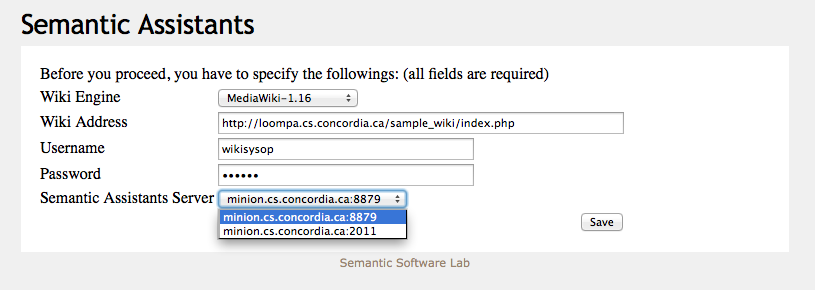
\includegraphics[width=0.9\textwidth]{pictures/wiki_config.png}
\caption{Configuring the Wiki-NLP integration}
\label{fig:wiki_config}
\end{figure}

Once the user saves the configuration, the provided information is stored in the user's browser and will remain for the consequent Wiki-SA interactions. The configuration page is only shown to users once, in the beginning of their session unless the cookies are explicitly removed by the user. Clicking on the ``Save'' button, will return the user to the previous page that the user was viewing.

\subsubsection{NLP Service Invocation}
Once the configuration settings are stored in the user's browser, users can inquire about the available NLP by clicking on the ``Semantic Assistants'' link the wiki menu bar. This action will reload the page, but this time the NLP user interface is appended to the bottom of the current wiki page. This user interface shown in Figure~\ref{fig:semassist_ui} allows the users to view a dynamically generated list of available assistants and select wiki pages of interest to a so-called ``collection''. The list pages in the collection is temporarily stored in the browser, hence, users can continue browsing to other pages of the wiki.

\begin{figure}
\centering
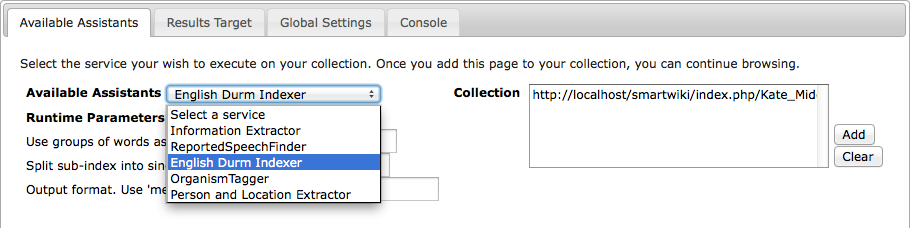
\includegraphics[width=\textwidth]{pictures/semassist_ui.png}
\caption{The Wiki-NLP interface in MediaWiki}
\label{fig:semassist_ui}
\end{figure}

Once the collection is prepared and an assistant is selected from the list, the second tab of the Wiki-NLP interface allows users to choose where they would like the results to be stored. Illustrated in Figure~\ref{fig:semassist_target}, the current available choices in the integration are:

\begin{itemize}\itemsep1mm
\item \emph{``Same Page''}, i.e., the results will be written in the same page as the resource. If the user has multiple pages in the collection, each results will be written into its corresponding source page. The current, option for this item are a wiki page's main ``body'', or its associated ``talk''\footnote{In some MediaWiki skins, a talk page is also known as the ``discussion'' page.} section.
\item \emph{``Another Page''}, i.e., writing the results to a different page in the wiki. If the user has multiple pages in the collection, the results of each wiki page will be aggregated into one output and written into the specified wiki page. In order to precisely choose a destination for this option, users have to select a namespace from a list of available namespaces in the wiki, as well as a type a unique page name. If the specified wiki page exists in the wiki, the results will be appended to the end of the page, otherwise a new wiki page will be automatically created.
\item \emph{Another Wiki} i.e., writing the results of the analysis into a different wiki than the source, provided that its engine is supported by the integration. Needless to say, users must provide the integration with (1) the address of the destination wiki, (2) its underlying wiki engine and version, (3) a valid username and password, and (4) a valid page name. Similar to the previous option, the results of the analysis will be aggregated and made persistent in the destination wiki page.
\end{itemize}

\begin{figure}
\centering
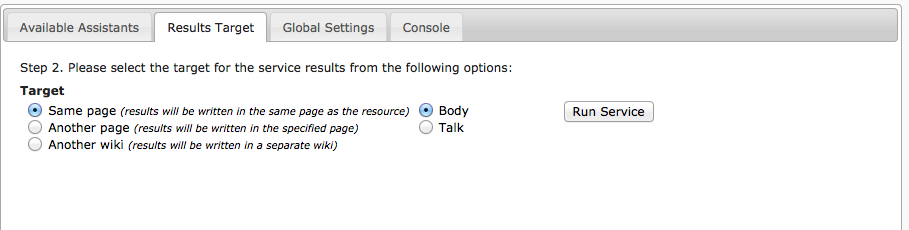
\includegraphics[width=\textwidth]{pictures/semassist_target.png}
\caption{The Wiki-NLP interface in MediaWiki}
\label{fig:semassist_target}
\end{figure}

The ``Console'' tab of the Wiki-NLP interface shows user-friendly logs of the NLP service execution and indicates where the results are written, if the execution is successfully done.

\subsubsection{Global Settings}
Similar to other \sa clients, users can dynamically change which \sa server they want their wiki to connect to. The ``Global Settings'' tab in the Wiki-NLP interface shown in Figure~\ref{fig:semassist_settings}, allows users to select a \sa server from a list of pre-defined addresses, as well as defining a custom end point. Once the user clicks the ``connect'' button, the selected server address is stored in the user cookies and will take effect as soon as the user refreshes the browser.

\begin{figure}[h!]
\centering
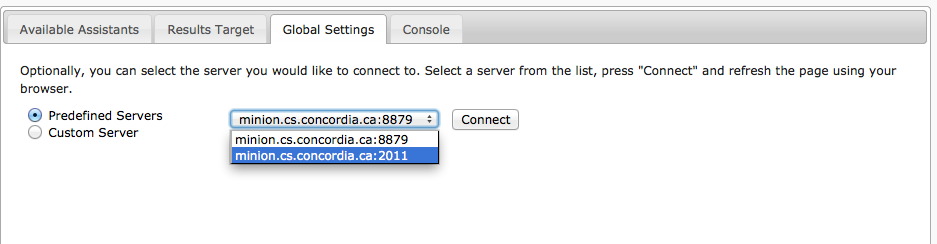
\includegraphics[width=\textwidth]{pictures/semassist_settings.png}
\caption{Global settings of the Wiki-NLP integration}
\label{fig:semassist_settings}
\end{figure}

\subsection{Installation}
The Wiki-SA integration is composed of two separate components: a server-side component and a wiki plug-in. While the server-side component is the same for different wiki systems, each wiki extension should be implemented for a specific engine. If you prefer to use the services available on our public repository, you can skip the next section and continue on to the wiki plug-in installation.

\subsubsection{Server-Side Component}
In order to install the server-side component, browse to \url{Clients/Wiki} folder in the \sa folder and type \texttt{ant pack}. This command will automatically build the server-side component as a \texttt{.WAR} file that can be deployed on any Java Servlet Container program, such as the Apache Tomcat. Deploying the servlet on a container varies from one program to the other. Please consult the user guide of your container of choice for this matter.

Once the server-side is deployed and started, it is automatically published on the container's default port number. For example, if your Tomcat is configured to use port \texttt{8080} as its default port, the servlet will be accessible on \texttt{http://HOSTNAME:8080/SA-WikiConnector}.

\subsubsection{Wiki Plug-in}
The Wiki-SA integration needs to be introduced to the wiki through a plug-in. Here, we will provide the details of installing the \sa extension for MediaWiki, available in \url{Clients/Wiki/MediaWiki/extension} folder. Simply copy the \texttt{\sa} folder to \url{PATH_TO_YOUR_MEDIAWIKI/extensions} folder. Next you have to \emph{install} the extension on the wiki engine by adding the following line to the \url{LocalProperties.php} file present in the root of your MediaWiki installation folder.

\begin{figure}[h!]
\centering
\begin{lstlisting}[language=PHP,numbers=left,xleftmargin=4mm,columns=flexible]
include_once("$IP/extensions/SemanticAssistants/SemanticAssistants.php");
\end{lstlisting}
\caption{Installing the \sa extension on the MediaWiki engine}
\label{list:mediawiki_sa_extension_install}
\end{figure}

Adding this line is all that is needed to enable your wiki user to inquire and invoke NLP pipeline on the wiki content. However, the extension by default connects the public \sa wiki component. If you have installed the server-side component described in the previous section, you have to change the default wiki component address to the servlet deployed on your container. Find the following line in \url{PATH_TO_YOUR_MEDIAWIKI/extensions/SemanticAssistants/SemanticAssistants.php} file and update in accordingly, by changing the \emph{``http://loompa.cs.concordia.ca:8080/''} to where your wiki component is published:

\begin{figure}[h!]
\centering
\begin{lstlisting}[language=PHP,numbers=left,xleftmargin=4mm,columns=flexible]
print("<li> <a href=\"http://loompa.cs.concordia.ca:8080/SA-WikiConnector/SemAssistServlet?action=proxy\">Semantic Assistants</a></li>");\end{lstlisting}
\caption{Configuring the \sa MediaWiki extension file}
\label{list:mediawiki_sa_extension_config}
\end{figure}

You can verify the successful installation of the \sa extension, by viewing the ``\texttt{Special:Version}'' page of your wiki: The \sa extension must be listed under the ``Installed extensions'' section of the page (Figure~\ref{fig:semassist_plugin} (a)), and a ``Semantic Assistants'' link is added to the wiki menu bar (Figure~\ref{fig:semassist_plugin} (b)).

\begin{figure}
\centering
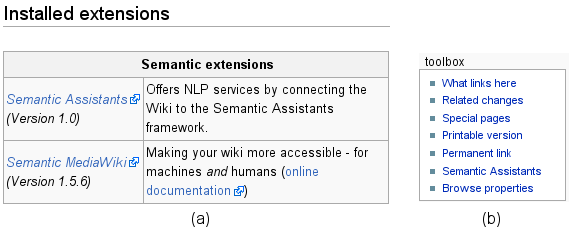
\includegraphics[scale=0.8]{pictures/semassist_plugin.png}
\caption{The \sa extension installed on MediaWiki}
\label{fig:semassist_plugin}
\end{figure}


\subsubsection{Wiki Templates}
The NLP pipelines results are made persistent in the wiki once the analysis is finished. For a more user-friendly results, there are pre-defined, customizable templates in the \sa Wiki-NLP integration that embed the generated results in a wiki table format. In order to use the templates in your MediaWiki instance, you have to import them to your wiki repository. Browse to the ``\texttt{Special Pages}'' page of your wiki and click on the ``\texttt{Import Pages}'' link under the ``\texttt{Page Tools}'' section\footnote{In the default installation of MediaWiki, permission of importing pages to the wiki is limited to users with the ``admin'' role.}. From the ``\texttt{Import XML data}'' box click on the ``\texttt{Browse}'' button and upload the \texttt{WikiNLP\_SA\_templates.xml} file located in the \url{Clients/Wiki/MediaWiki/templates} folder, as shown in Figure~\ref{fig:wiki_template_import}.

\begin{figure}
\centering
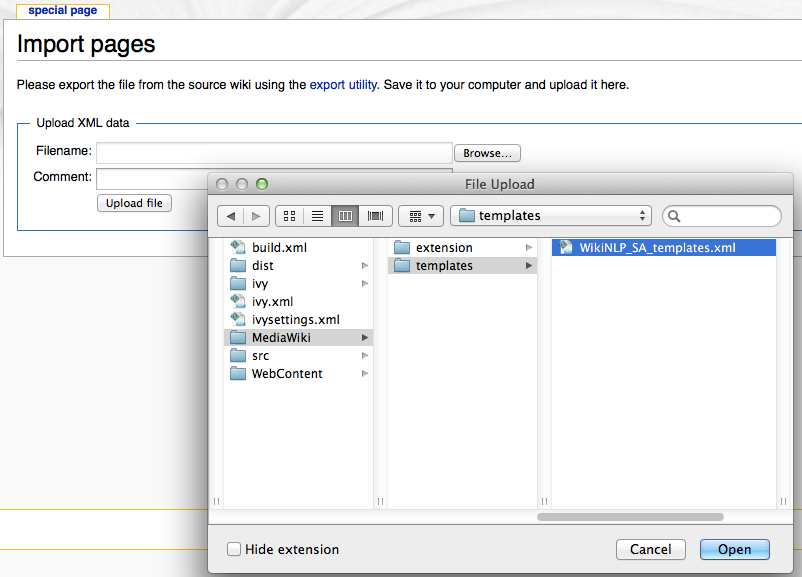
\includegraphics[width=0.9\textwidth]{pictures/wiki_template_import.png}
\caption{Importing the \sa templates to MediaWiki}
\label{fig:wiki_template_import}
\end{figure}

Note that there are no templates for the ``File'' and ``Document'' output types (see Section~\ref{sec:response}) and the content of the generated output is written to the wiki repository as regular wiki pages.

\subsection{Development Notes}
In this section, we provide further details on the underlying architecture of the Wiki-NLP architecture and how more wiki engines can be added to the integration.

\subsubsection{System Architecture}
As stated earlier, the Wiki-NLP architecture is a collaborative approach, combining the power of an extensible server-side component and a lightweight wiki-side plug-in. While the server-side wiki component is responsible for executing the NLP services, the wiki extension handles all the wiki-specific tasks, such as manipulating the wiki menu bar or patrolling changes in the wiki repository. In our system architecture, illustrated in Figure~\ref{fig:wikinlp_arch},the communication between the two aforementioned components and the user's browser is carried out over the HTTP protocol using JavaScript code that is dynamically injected into the user's browser.

\begin{figure}
\centering
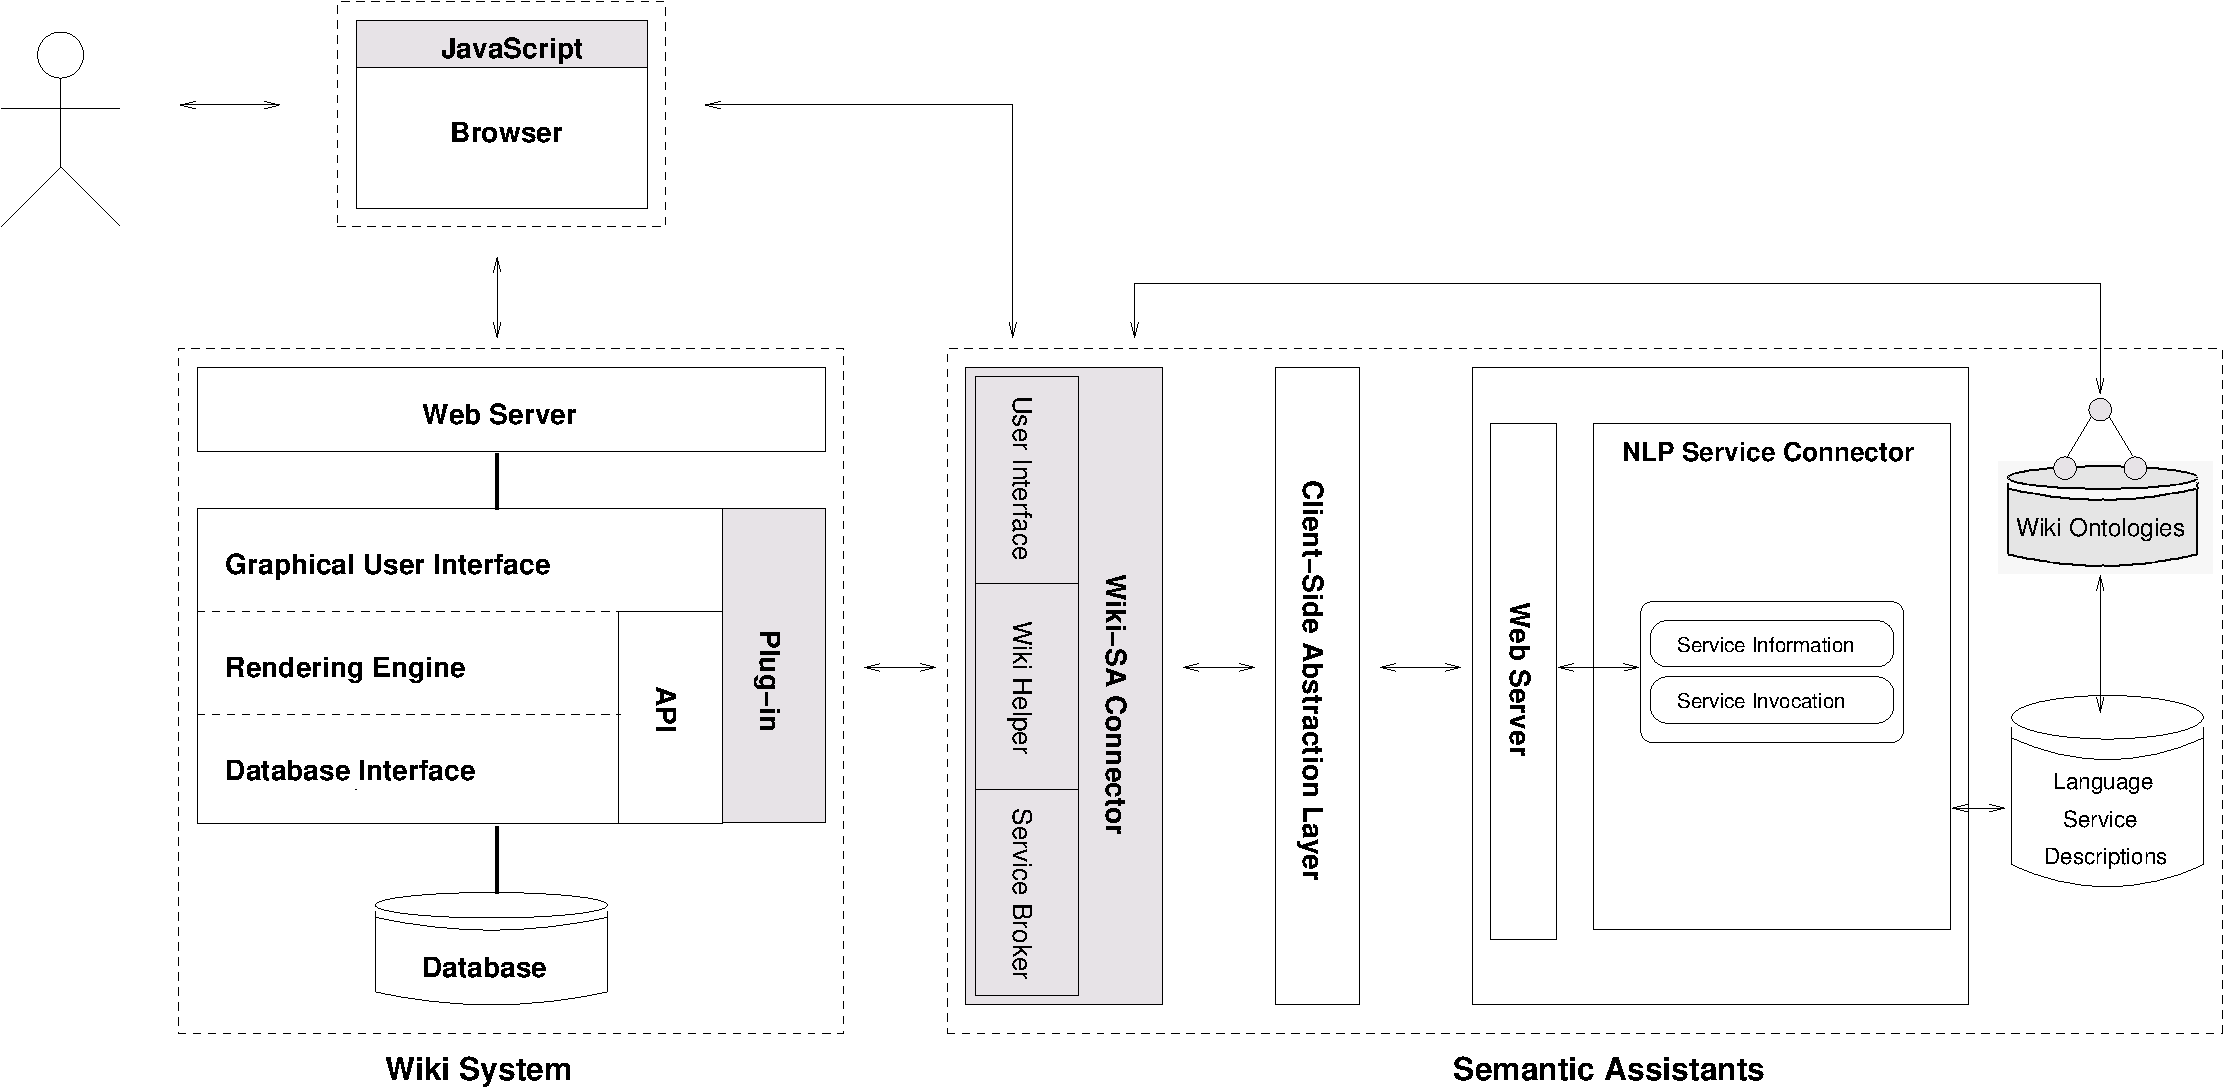
\includegraphics[width=0.9\textwidth]{pictures/wikinlp_arch}
\caption{The Wiki-NLP integration architecture}
\label{fig:wikinlp_arch}
\end{figure}

An analysis session is started when the user clicks on the \sa link in the wiki, like the one shown in Figure~\ref{fig:semassist_plugin}, or the wiki extensions makes a headless request to the wiki component. If the request parameters are not sufficient, the user is redirected to the settings page. Otherwise, the wiki component loads the requesting wiki ontology from its repository (see the next section) and generates a custom user interface based on the wiki capabilities, e.g., its list of namespaces, etc. The user interface is then injected into the user's browser, as shown in Figure~\ref{fig:semassist_ui}.

Once an NLP service execution is sent to the wiki component, the service call is delegated to the designated \sa server and the results are transformed and written back to the wiki repository.

\subsubsection{Wiki Ontologies}

we adopted a semantics-based approach, in which different wiki engines are introduced to the integration architecture through their \emph{ontology} files. By using OWL as the ontology language to formally describe a wiki, the integration does not need to know about their concrete implementation; rather it uses automatic reasoning on their ontologies to discover each wiki's structure and capabilities.

\begin{figure}
\centering
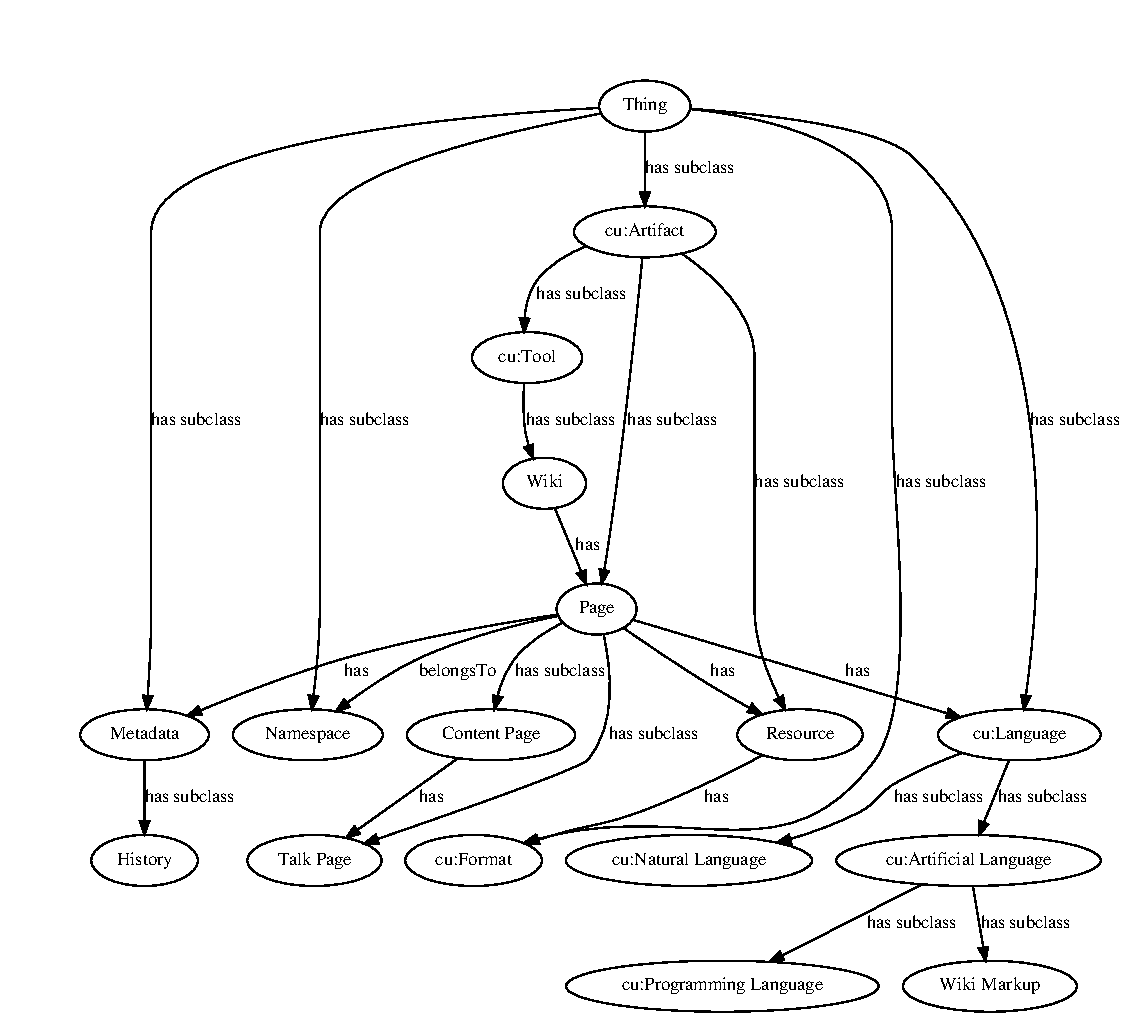
\includegraphics[scale=0.7]{pictures/wiki_onto.pdf}
\caption{Wiki Upper Ontology}
\label{fig:wiki_onto}
\end{figure}

To facilitate the process of ontology definition, we have designed a generic \emph{upper ontology} for wiki systems shown in Figure~\ref{fig:wiki_onto}, which also includes concepts defined in the \sa upper ontology~[\cite{aswc08}] -- a multi-purpose ontology that describes five core concepts to model the relationships between users, their tasks, the artifacts involved and their format and language.  

\begin{table}
\centering
\caption{Concepts in the wiki upper ontology}
\label{tab:wiki_onto_concepts}
\textsf{\small
\begin{tabular}{l l l}
  \hline 
  \textbf{Concept}&\textbf{Description} &\textbf{Example} \\
  \hline
  Wiki & \emph{wiki engine}  & MediaWiki
  \\
  Page & \emph{Wiki elements encompassing textual content} & ``Semantic Web''
  \\
  Namespace & \emph{Category names to differentiate pages at a high level}  & ``Help'', ``Project''
  \\  
  Resource & \emph{Files with arbitrary formats} & Picture.jpg
  \\
  Metadata & \emph{Metadata associated with wiki pages}  & History, Semantic Annotations
  \\
  Wiki Markup & \emph{Ontological representation of wiki syntax} & MediaWiki Markup\\
\hline
\end{tabular}}
\end{table}

The wiki upper ontology is designed using Prot\'{e}g\'{e}\footnote{Prot\'{e}g\'{e}, \url{http://protege.stanford.edu/}} and reflects the concepts that are common to all wiki engines. Thus, for the MediaWiki engine, we merely have to instantiate the upper ontology manually or automatically using special scripts to define the concrete structure of each wiki instance, e.g., its available namespaces. Table~\ref{tab:wiki_onto_concepts} summarizes the concepts of the wiki upper ontology.

\subsubsection{Results Transformation and Presentation}
The ultimate goal of our Wiki-NLP integration is to create a ``self-aware'' wiki that can develop and organize its content. Therefore, unless the results from NLP services are presented to users or become persistent in the wiki, the integration would not add any valuable advancement to the current state of the underlying wiki system. Transforming the NLP service results to wiki markup is a task handled by special parser classes in the wiki helper module described in the previous section.

\begin{figure}[h!]
\centering
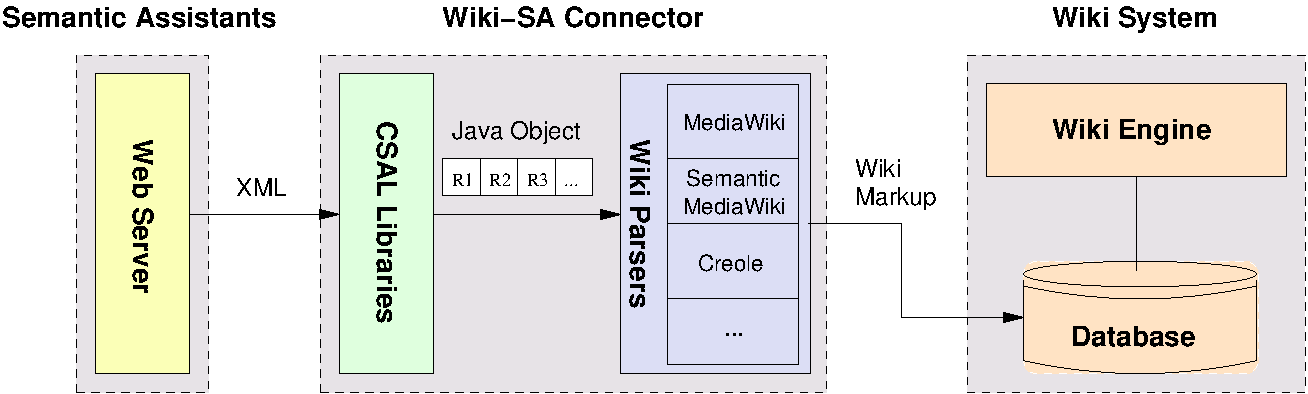
\includegraphics[width=0.7\columnwidth]{pictures/result_transform.pdf}
\caption{Transforming NLP service results to wiki markup}
\label{fig:result_transform}
\end{figure}

Following a successful NLP service execution, results are passed from the \sa server to the service broker module in form of an XML message (see Figure~\ref{list:response1} for an example). The wiki component then interprets the server's XML response and parses the message into an array of Java objects. The service result objects are then transformed to wiki markup by the wiki helper classes in the wiki component and prepared for the \emph{templating mechanism}. 

The templating mechanism is the process of embedding service results into MediaWiki templates for presentation. This mechanism separates the data model from its presentation and provides the opportunity to create multiple views for a single model for different purposes. Templating is a collaborative task performed by the wiki component and the wiki extension. The wiki component prepares the markup by placing the results within their corresponding templates and storing them in the wiki's database. Once the wiki page is viewed by the user, the templates installed on the wiki by the \sa extension will render the template markup to generate appropriate HTML representations for NLP results, such as tables or lists. Figure~\ref{fig:result_transform} shows the workflow of the transformation of server XML response messages to MediaWiki markup.

\subsubsection{Wiki Component Structure}
The Wiki-SA Connector component, shown in Figure~\ref{fig:wikinlp_arch}, is technically an HTTP proxy sever written using the Java Servlet\footnote{Java Servlet API, \url{http://download.oracle.com/docs/cd/E17802_01/products/ products/servlet/2.5/docs/servlet-2_5-mr2/}} technology. As mentioned earlier, it acts as an intermediator between the \sa server, the wiki system and the user's browser by intercepting their communication. For each of these three endpoints, there exists a module in the servlet, specifically concerned with the endpoint's business logic. This way, having separate modules allows the sub-components to evolve and extend independently.

\blankline
\noindent
\textbf{Service Broker Module. }{The service broker module is the connecting point of the integration to the \sa server. Every service execution request that is received by the integration component is translated into a Java method call in this module, which in turn triggers the execution of one or multiple NLP services in the \sa server.}

\blankline
\noindent
\textbf{User Interface Module. }{This module is responsible for generating the integration user interface within a wiki environment. Since wikis are accessible through Web browsers, this module is designed to generate an HTML representation of the Semantic Assistants user interface and inject it to the the user's browser using JavaScript. Figure~\ref{fig:semassist-ui} shows how the generated user interface is added to a wiki page to give its users the impression that they are still interacting with the wiki's native interface. Through this user interface, users can find the \emph{Available Assistants} (bottom left) and invoke arbitrary NLP services by dynamically querying the \sa repository of service descriptions. This way, any language service that is offered by a \sa server is presented in the user interface to the user. Moreover, the generated user interface allows users to combine multiple pages of the wiki in a \emph{collection}, i.e., a list of user-selected page URLs, and invoke the NLP service on them at once.}

\blankline
\noindent
\textbf{Wiki Helper Module. }{The wiki helper module encompasses the classes required for communicating with the MediaWiki engine. The classes in this module are responsible for providing the NLP pipelines with input data by reading wiki pages from the database and eventually transforming the results to their corresponding template markup and storing them in the wiki database.}


Earlier we stated that the wiki component is responsible for maintaining and reasoning on the available wiki ontologies. This process is achieved by special ontology keeper classes that upon each servlet bootstrapping, run over the wiki repository OWL files and create an in-memory model of the wikis, by parsing them using Prot\'{e}g\'{e}'s OWL libraries. This module also provide reasoning capabilities on wiki ontologies using the SPARQL\footnote{SPARQL Query Language for RDF, \url{http://www.w3.org/TR/rdf-sparql-query/}} language.

\subsubsection{Extending the Wiki Component}
One main requirement in the design of Wiki-NLP is wiki independence. With this requirement in mind, we have realized an extensible architecture where wikis can be added to the integration wiki little effort. The directory structure of the server-side wiki component found in \url{Clients/Wiki/src/info/semanticsoftware/semassist/client/wiki} is as follows:

\begin{enumerate}
\item\url{broker}: This folder contains the classes that handle the NLP service execution in the \sa server, as well as partial refinement of the results.
\item\url{command}: This folder contains classes pertaining to the Factory Design Pattern that generate various commands that the servlet can handle. The commands themselves are implemented using the Command Design Pattern. 
\item\url{html}: This folder contains classes that generate an HTML representation of the Wiki-NLP user interface.
\item\url{servlets}: This folder contains the front controller classes in our proxy design.
\item\url{utils}: This folder contains utility classes related to the wiki component, such as logging and abstract parser classes.
\item\url{wikihelper}: This folder contains the classes pertaining to the Factory Design Pattern that generate various wiki engine instances and their corresponding parsers on the fly. Essentially, the Wiki-NLP integration provides three abstract classes, namely, \texttt{WikiHelper.java}, \texttt{WikiParser.java}, \texttt{WikiOntolgyKeeper.java}, that provide abstract methods to communicate with the wiki engine, transform the results to wiki markup and query the wiki ontology files, respectively. 
\end{enumerate}

As the directory structure suggests, in order to introduce a new wiki engine to the integration architecture, the three mentioned classes in the \texttt{wikihelper} package needs to be extended. The current \texttt{wikihelper} package contains example classes for the MediaWiki engine. Similarly, if your wiki engine is called XWiki, you need to create \texttt{XWikiHelper.java}, \texttt{XWikiParser.java} and \texttt{XWikiOntologyKeeper.java} classes that extend the corresponding abstract classes. Oncee these three classes are implemented, simply extend the factory pattern in the \texttt{WikiFactory.java} by adding the name of your wiki engine to the switch statement, as shown in Figure~\ref{list:wiki_factory_extend}:

\begin{figure}[h!]
\centering
\begin{lstlisting}[language=Java,numbers=left,xleftmargin=4mm,columns=flexible]
  /** Enumeration class for Servlet commands. */
  enum Wikis {mediawiki, xwiki};

  public static WikiEngine getWiki(final String engine){
    switch(Commands.valueOf(command.toLowerCase())){
		case proxy:
			return new MediaWiki();
		case params:
			return new XWiki();
		default:
			return null;
		}
  }
\end{lstlisting}
\caption{Extending the wiki factory class}
\label{list:wiki_factory_extend}
\end{figure}

Next, create a class called \texttt{XWiki.java} and reference a singleton access to your wiki helper, parser and ontology keeper classes, just like the code in \texttt{MediaWiki.java}. Finally, place your wiki ontology \texttt{.owl} file in \url{Clients/Wiki/WebContent/ontology-repository} folder and your wiki will show up in the list of supported engines once the servlet is restarted.

\section{Android Application}
Mobile phones use a variety of operating systems that transform them from a traditional handheld device for talking into general-purpose computing platforms. Android OS\footnote{Google's Android Platform~\url{http://developer.android.com}}, is an open source platform for mobile and tablet development led by Google Inc. It is a comprehensive Linux-based platform that supports most of the Java Platform and features its own extensive user interface framework. This platform is widely used by programmers to create applications and games for handheld devices. We have leveraged this platform to create an application that allows users to use novel NLP solutions inside their devices. This app, henceforth referred to as the \sa App, not only can be used as a standalone application, but also plays the role of a system-wide NLP service provider for other applications. Note that the \sa App was originally implemented based on Android 3.0 Platform\footnote{Android 3.0 Platform,~\url{http://developer.android.com/sdk/android-3.0.html}} (Honeycomb) but its backward compatibility has also been tested with Android 2.2. It is, however, recommended that the app be used in Android 3.0+ versions.

In the following sections, we describe the \sa App features and provide a guide on how to use the \sa App services inside external applications.

\subsection{Features}
The user interface shown in Figure~\ref{fig:android_main} is the \sa main activity (user interface). This means that once the app is installed on the device, this is the main entry to the application. It allows users to connect to a specific \sa server and invoke an assistant on the provided text input.

\begin{figure}[htb]
\centering

\includegraphics[scale=0.35]{pictures/android_main.jpg}
\caption{\sa Android App Main Activity}
\label{fig:android_main}
\end{figure}
\subsubsection{\sa Account}
Each android-enabled device has at least one built-in account type, i.e., the Google account. Android is designed in such a way that the same account can be registered to a variety of account-based services. For example, the Gmail account that is set up on the Android device is not just used for e-mailing , but for all the Google account-based applications. The same concept applies to the \sa App that uses the \emph{\sa account} type for its applications. Just like another accounts, you first need to sign up for a \sa Account before using the application.

Once you have obtained your credentials, on your device browse to \texttt{Settings $\rightarrow$ Accounts and Sync $\rightarrow$ Add Account} and choose the ``\sa'' option from the list. In the provided user interface, type in your \sa accounts credentials and press \texttt{Sign in}. If authenticated successfully, your \sa account will appear in the list of your device accounts.

\blankline
\noindent
\textbf{Note:} Before authenticating or signing up for an account, you need to choose the \sa server where your account is located. For this, follow the instructions in Section~\ref{sec:android_global_settings}.

\subsubsection{Global Settings}
\label{sec:android_global_settings}
Similar to other \sa clients, the \sa App allows users to connect to various arbitrary servers to inquire about their available assistants. On the \sa App main activity, press the \texttt{Global Settings} button. The application settings activity will pop up that allows you to define a new server location or choose one from a list of available servers as shown in Figure~\ref{fig:android_global_settings}.

\begin{figure}[htb]
\centering
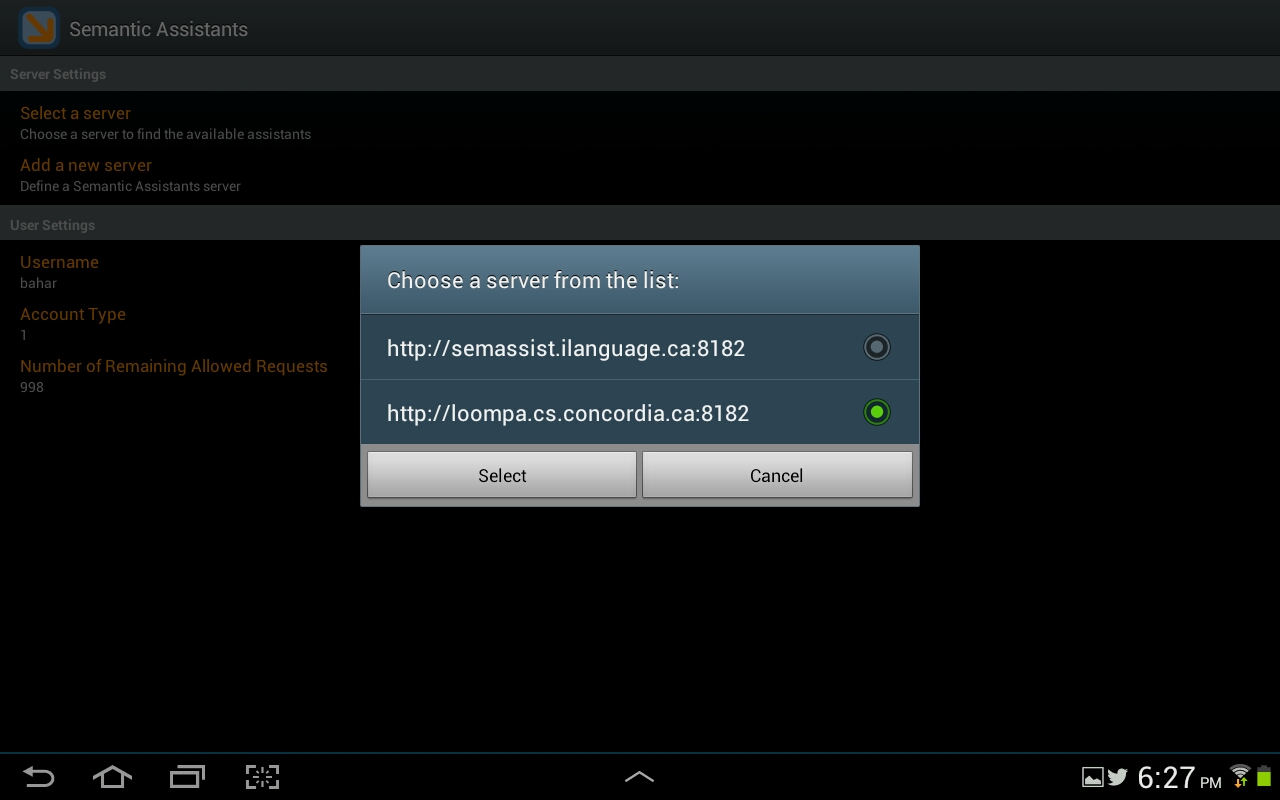
\includegraphics[scale=0.35]{pictures/android_global_settings.jpg}
\caption{\sa App Global Settings Activity}
\label{fig:android_global_settings}
\end{figure}

In order to add a new server location, click on the \texttt{Add a new server} option and type in the server URL by concatenating the server address, including its protocol and port number, like in Figure~\ref{fig:android_new_server}. In order to choose the newly defined server, choose the \texttt{Select a server} option from the Global Settings activity and select it from the list.

\begin{figure}[htb]
\centering
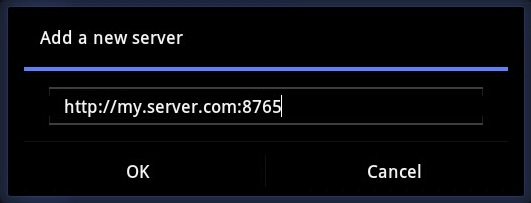
\includegraphics[scale=0.5]{pictures/android_new_server.jpg}
\caption{Adding a new server to the \sa App settings}
\label{fig:android_new_server}
\end{figure}

\subsubsection{NLP Service Invocation}
Once the \sa server is selected from the Global Settings activity, users can inquire about its available assistants. From the \sa App main activity, press the \texttt{Available Assistants} button to open the service invocation activity. This activity, as shown in Figure~\ref{fig:android_invoke_main}, presents the list of available assistants and an input text area for the text to be analyzed. By selecting each assistants from the list, the app will provide detailed information of what the assistant does and allows to customize the pipeline execution through providing runtime parameters.

\begin{figure}[htb]
\centering
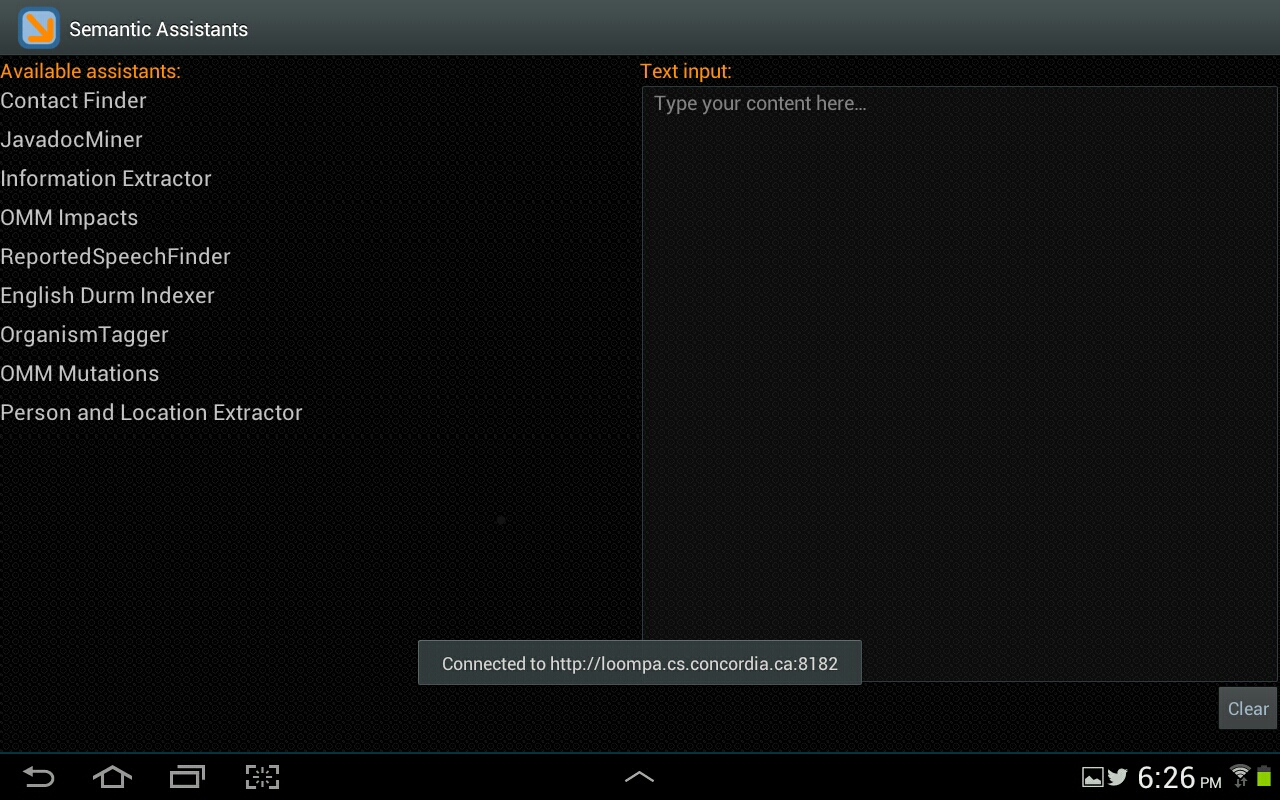
\includegraphics[scale=0.35]{pictures/android_invoke_main.jpg}
\caption{Invoking an NLP service through the \sa App settings}
\label{fig:android_invoke_main}
\end{figure}

Users have three options on how to provide a pipeline with text input:
\begin{itemize}
\item{\textbf{Manually typing in the text. }}{Using the device keyboard, type in the text that is to be analyzed.}
\item{\textbf{Sharing text with the \sa from other apps. }}{The \sa App listens for sharing event in the Android platform. This means that from within applications that provide a sharing mechanism, the selected text can be directly placed into the \sa Apps activity input.}
\item{\textbf{Sending input to the \sa service. }}{As we will explain more in Section \ref{sec:android_service}, the text input can be sent via a service argument (extra). The difference between this option and the previous bullet is that in the sharing option, the \sa App takes care of the result handling instead of the invoking application. Also in this service invocations, the NLP service to be executed is pre-defined and cannot be changed at a later stage.}
\end{itemize}
Once done with typing, select an assistants from the left-side list and press the \texttt{Invoke} button. Depending on the type of the results, you would either see the annotations in a new activity or the resulting file will be opened in the device browser.

\subsection{Installation}
TBD

\subsection{\sa App Service}
\label{sec:android_service}
As mentioned earlier, the \sa App also plays the role of a system-wide service provider, meaning that other external applications can use the \sa App's functionality. This is done through using Android services, i.e., application components that can perform long-running operations in the background. Each available service in the \sa App has a unique name that should be indicated when the external application invokes the service.

To better demonstrate this feature, we will illustrate a demo app that uses a \sa service. The demo in example, called iForgotWho, is an app that helps users to find potential ``contacts'' from a given text and upon user accept, automatically adds them to the device contact book. However, the iForgotWho app does not find the contacts by itself, rather it uses the \sa App's \texttt{person\_extractor} service. For this, the iForgotWho needs to (1) invoke the service using its complete identifier (available in the \sa App manifest file), (2) send along the text to be analyzed, and (3) indicate whether the \sa App should present the results or iForgotWho takes care of it. Once all the data is provided to the \sa App, the NLP service is executed and the results are passed back to iForgotWho app. Then, iForgotWho presented the list of all the person entities found in the text to the user, whom which ultimately decide whether they should be added to the device contact book. Figure~\ref{fig:android_service} illustrates this sequence.

\subsection{Development Notes}
In this section, we provide technical notes about the \sa App and how external Android application developers can integrate NLP capabilities in their apps using the \sa services.

\subsubsection{Extending the \sa App}
The \sa App source directory is structured as follows:
\begin{enumerate}
\item\url{activity}: This folder contains the classes representing graphical user interfaces.
\item\url{application}: This folder contains the \sa App's main application class and provides a static access to its context.
\item\url{business}: This folder contains the classes that handle communication with the \sa server.
\item\url{encryption}: This folder contains classes that take care of the secure HTTP connection attributes, such as the SSL certificate.
\item\url{intents}: This folder contains the intents factory class used by \sa App's services.
\item\url{parser}: This folder contains the parsers for Restful request and response representations.
\item\url{prefs}: This folder contains the utility classes for Android preference management.
\item\url{service}: This folder contains the authentication and service invocation service listeners.
\item\url{utils}: This folder contains the app's utility classes.
\end{enumerate}

In order to extend the \sa App, import the \sa App to your Eclipse or other IDE of choice. Note that you need to have the Android SDK\footnote{Android SDK, \url{http://developer.android.com/sdk/}} specific to your operating system installed on your machine.

\subsubsection{Using the \sa App Service}
In order integrate the \sa App service in your application, you have to first find the exact service name in the \sa App's manifest. For example, in order to detect Person named entities in a text, you have to call the \texttt{org.openintents.action.PERSON\_EXTRACTOR} service, using this code:

\begin{lstlisting}[language=Java,numbers=left,xleftmargin=4mm,columns=flexible]
 // specify which service should be invoked
 Intent service = new Intent(org.openintents.action.PERSON_EXTRACTOR);

 // the text to be analyzed
 String input = "I met John Smith at a conference last year.";

 // set the service input
 service.putExtra(Intent.EXTRA_TEXT, input);

 // let the Semantic Assistants App know the invoking app will present the results
 service.putExtra("SILENT_MODE", "true");

 // call the service
 startService(service);
\end{lstlisting}

You also have to define a Broadcast Receiver\footnote{Android Broadcast Receiver, \url{http://developer.android.com/reference/android/content/BroadcastReceiver.html}} to get back the results from the \sa App once the service results are ready. In your broadcast receiver class, you can then decide on how to present the results. Note that what the \sa App returns is the XML representation of the NLP pipeline as discussed in Section~\ref{sec:response}.

\subsubsection{Adding More ServiceIntents}
You can also easily add more services to the \sa App. In order to add a new service you must take the following steps:

\blankline
\noindent
\textbf{Step 1: Add the service name to list of available services. } In order to inform the \sa App of the newly added service, you need to add the unique name of the service as an \texttt{intent-filter} to the \texttt{service} node in the \sa App's manifest file. Specifically, you should add these lines to the \texttt{AndroidManifest.xml} file:

\begin{lstlisting}[language=XML,numbers=left,xleftmargin=4mm,columns=flexible]
<service android:name="info.semanticsoftware.semassist.android.service.SemanticAssistantsService"
		 android:process=":semassist_service" 
		 android:label="semassist">
	<intent-filter android:label="A_LABEL_FOR_YOUR_SERVICE">
		<action android:name="com.example.action.YOUR_SERVICE_NAME" />
		<category android:name="android.intent.category.DEFAULT" />
	</intent-filter>
</service>
\end{lstlisting}

Adding this line to the manifest allows the \sa App to receive the service requests from external applications.

\blankline
\noindent
\textbf{Step 2: Create the class that handles the results. }
Next is to create the class that will perform the actual service execution and handles the server response. This new class must extend the \texttt{ServiceIntent} class in the \texttt{intents} package and must have a \texttt{execute{}} method. In your execute method, you should let the parent class handle the actual service execution and instead handle the response before sending it back to the invoking app. The following snippet shows the service class for the \texttt{PERSON\_EXTRACTOR} service:

\begin{lstlisting}[language=Java,numbers=left,xleftmargin=4mm,columns=flexible]
public class PersonExtractorIntent extends ServiceIntent{

	// the exact service name as specified in its OWL file
	private final static String PR_NAME = "Person and Location Extractor";

	public PersonExtractorIntent(){
		super(PR_NAME);
	}

	public String execute() {
		//STEP1: Execute the service
		String rawResults = super.execute();

		//STEP2: Filter the results
		try{
			String filteredResult = "";
			// remove anything but "Person" annotations from the rawResults
			...
		} catch (Exception e){
			// handle exception
			....
		}
		return filteredResults
	}
}
\end{lstlisting}

\blankline
\noindent
\textbf{Step 3: Update the factory class. }
Finally let the \texttt{ServiceIntentFactory} class know how to map a service request to its corresponding handling class by adding the service action name to its enumeration class:

\begin{lstlisting}[language=Java,numbers=left,xleftmargin=4mm,columns=flexible]
/** Enumeration class for service intents */
enum Intents {person_extractor, YOUR_SERVICE_NAME};
\end{lstlisting}

\blankline
\noindent
and update the switch statement:

\begin{lstlisting}[language=Java,numbers=left,xleftmargin=4mm,columns=flexible]
switch(Intents.valueOf(action.toLowerCase())){
	case person_extractor:
		return new PersonExtractorIntent();
	case your_service_name
		return new YourServiceIntent();
	default:
		return null;
	}
\end{lstlisting}

\section{Global Preference Management}
\label{sec:pref_management}
Semantic Assistants clients preferences are stored in a single hidden file in the user machine's home directory under the name \texttt{semassist-settings.xml}. This file is shared between all the clients and contains information, such as different servers that clients can connect to as well as other client-specific preferences. The preference XML document has two main parts: a global part and a client-specific part. The scope of the global preference, as the name suggests, is all of the clients and any changes to this part will affect them all. The client-specific scope, on the other hand, is limited to that specific client and does not affect others. Each Semantic Assistants client installed on the user machine has a dedicated tag inside the client-specific part, where it can store its proprietary preferences.

This file does not ship with the Semantic Assistants project but a default preference file is created by the very first client installed and used on the user's machine and will be reused by the subsequent clients. It is not advised to manually modify this file unless its structure can be kept consistent. In case of deletion, a default file will be again created by the next used client. The structure of the preference file is detailed in \ref{client_pref}.